% Share this document for others to view with this URL
% https://www.overleaf.com/read/cvfmtqkfphmr#384bf0
%
\documentclass{article}

%--------------------
% PACKAGES
\usepackage[utf8]{inputenc} % allow utf-8 input
\usepackage[T1]{fontenc}    % use 8-bit T1 fonts

\usepackage[pagebackref]{hyperref} % hyperlinks
\usepackage{url}            % simple URL typesetting

\usepackage[dvipsnames,table]{xcolor} % colors

\usepackage{graphicx}       % Required for inserting images
\usepackage{booktabs}       % professional-quality tables
\usepackage{multicol}       % cells spanning multiple columns
\usepackage{multirow}       % cells spanning multiple rows
\usepackage{makecell}       % multiline cells, etc
\usepackage{colortbl}       % colours in tables
\usepackage{caption}        % caption package
\usepackage{subcaption}     % make subfigures with their own graphics and own captions (a), (b), etc.
\usepackage{wrapfig}        % can make a figure only use part of the column width, text wraps around it
\usepackage{adjustbox}      % nice package for shrinking too-wide tables down (cleaner than using \resizebox)
\usepackage{titletoc}       % table-of-contents management, allowing a TOC for just appendix matter

\usepackage{mathtools}
\usepackage{amsmath,amsthm} % nice mathematics display
\usepackage{amsfonts}       % blackboard math symbols
\usepackage{amssymb}        % for the checkmark symbol
\usepackage{nicefrac}       % compact symbols for 1/2, etc.
\usepackage{microtype}      % microtypography

\usepackage{algorithm,algorithmicx,algpseudocode}

%\usepackage{pdflscape}      % support for landscape PDF pages (rotated pages)
\usepackage{comment}        % provides comment environment (use to suppress LaTeX)
\usepackage{array}
% \usepackage{times}         % Set default font to Adobe Times Roman

\usepackage{doi}            % provides nice \doi command
\usepackage[normalem]{ulem} % provides strikeout with \sout
\usepackage{placeins}       % provides \FloatBarrier
\usepackage[detect-all]{siunitx} % provides \num, \SI and other SI unit commands

% Configure packages
%~~~~~~~~~~
% Configure captions to be small, with label in italic
\captionsetup{font=small,labelfont=it}
% You can configure DOIs to be in smallcaps with a thin space, instead of lowercase without a space
% \renewcommand{\doitext}{{\scshape doi:\,}}

%--------------------
% SYMBOLS

% For frozen/unfrozen icons
%
% If you are not using the "unfrozen" icon, please comment out its code and delete file icons/SPB_flame.pdf
%
% Snowflake: U+008acd
\usepackage{bbding}         % provides some symbols
\definecolor{cold}{HTML}{008acd}
\def\frozen{\raisebox{-.15ex}{\color{cold}\SnowflakeChevron}}
\DeclareUnicodeCharacter{2744}{\frozen}% ❄, you can use the unicode in latex source, but it looks like * so don't - just use \frozen instead
%
% Fire: U+1F525
% https://commons.wikimedia.org/wiki/File:SPB_flame.svg
% CC BY-SA 4.0 Anton Landao, editted by Scott C. Lowe (change: colourized, #cd1600)
% \def\unfrozen{\raisebox{-.15ex}{\includegraphics[height=1em]{icons/SPB_flame.pdf}}}
\DeclareUnicodeCharacter{1F525}{\unfrozen}% ��, unicode symbol not currently supported on overleaf; just use \unfrozen instead

% Cross-mark (xmark) to use in tables like \checkmark
\usepackage{pifont}         % provides some symbols
\def\cmark{\ding{51}} % Alternative to \checkmark
\def\xmark{\ding{55}}
\definecolor{vlightgray}{gray}{0.87}
\def\myxmark{{\color{vlightgray}\xmark{}}}
\def\correctmark{{\color{ForestGreen}\cmark{}}}
\def\incorrectmark{{\color{red}\xmark{}}}

%--------------------
% COLOURS

% Tableau colors
\definecolor{tblue}{HTML}{1F77B4}
\definecolor{torange}{HTML}{FF7F0E}
\definecolor{tgreen}{HTML}{2CA02C}
\definecolor{tred}{HTML}{FF0000}

% Change links to be signified by text colour instead of in boxes
% We use colours that are similar to the default box colours by link type
%
% Colours based on Phelype Oleinik's colours
% https://tex.stackexchange.com/a/525297/108091
% but with modifications to those by Scott
\definecolor{linkcolor}{HTML}{991408}  % red
\definecolor{citecolor}{HTML}{2E7E2A}  % green
\definecolor{filecolor}{HTML}{131877}  % dark blue
\definecolor{menucolor}{HTML}{727500}  % yellow
\definecolor{runcolor} {HTML}{137776}  % teal
\definecolor{urlcolor} {HTML}{0a2bbf}  % blue
%
% Just comment out this \hypersetup command if you want to revert to boxes
\hypersetup{colorlinks=true,linkcolor=linkcolor,citecolor=citecolor,filecolor=filecolor,menucolor=menucolor,runcolor=runcolor,urlcolor=urlcolor}
%
% An alternative option is to make all links blue:
%\hypersetup{colorlinks=true,linkcolor=urlcolor,citecolor=urlcolor,filecolor=urlcolor,menucolor=urlcolor,runcolor=urlcolor,urlcolor=urlcolor}

%--------------------
% SPACE ADJUSTMENTS

% less space for equations
%\expandafter\def\expandafter\normalsize\expandafter{%
%    \normalsize%
%    \setlength\abovedisplayskip{2pt}%
%    \setlength\belowdisplayskip{2pt}%
%    \setlength\abovedisplayshortskip{-8pt}%
%    \setlength\belowdisplayshortskip{2pt}%
%}

%--------------------
% MACROS

% Referring to sections nicely
\renewcommand{\sectionautorefname}{Section}
\let\subsectionautorefname\sectionautorefname
\let\subsubsectionautorefname\sectionautorefname
\newcommand{\appref}[1]{\hyperref[#1]{Appendix~\ref*{#1}}}% For referencing subsections of the appendix

% Concise references
\def\Snospace~{\S{}}% Provides § without a space after it, so it butts up against section numbers
% Uncomment these commands to save space, or if you just like using the section symbol (§)
%\renewcommand*{\sectionautorefname}{\Snospace}
%\renewcommand*{\subsectionautorefname}{\Snospace}
%\renewcommand*{\subsubsectionautorefname}{\Snospace}
%\renewcommand*{\appref}[1]{\hyperref[#1]{App.~\ref*{#1}}}
%\renewcommand*{\figureautorefname}{Fig.}
%\renewcommand*{\equationautorefname}{Eq.}
%\renewcommand*{\tableautorefname}{Tab.}

% A paragraph command that is like a subsubsubsection
\newcommand{\mypara}[1]{\noindent\textbf{#1}}

% Writing links with the URL written out in a footnote
\newcommand{\hreffoot}[2]{\href{#1}{#2}\footnote{\url{#1}}}

% Results highlighting
\newcommand{\best}[1]{\textbf{#1}}
\newcommand{\secbest}[1]{\underline{#1}}
\newcommand{\runnerup}[1]{\secbest{#1}}

% Proofing
\newcommand{\hider}[1]{}
\newcommand{\TODO}[1]{\textcolor{red}{[\textbf{TODO}: #1]}}

\newtheorem{theorem}{Theorem}
\theoremstyle{definition}
\newtheorem{definition}{Definition}
\input{math_commands}


\usepackage{tikz}
\usetikzlibrary{positioning,arrows.meta,shapes.geometric,decorations.pathreplacing}

\tikzset{
  maincircle/.style={circle, draw, minimum size=13mm, inner sep=2pt, font=\footnotesize, align=center},
  fwd/.style={->, thick, >=Latex},
  promise/.style={->, dashed, thick, >=Latex,
                  preaction={draw, white, line width=3pt}}, % halo for visibility
  diamondnode/.style={diamond, draw=green!60, fill=green!5, very thick, minimum size=7mm},
  node/.style={circle, draw=green!60, fill=green!5, very thick, minimum size=7mm},
  orange/.style={draw=orange!60, fill=orange!5},
  red/.style={draw=red!60, fill=red!5},
  blue/.style={draw=blue!60, fill=blue!5},
  teal/.style={draw=teal!60, fill=teal!5},
  purple/.style={draw=purple!60, fill=purple!5},
  highlight/.style={ultra thick},
}
\usepackage{natbib}
\usepackage{etoolbox}       % Provides toggle
\newtoggle{arxiv}% Swap between arXiv and journal/conference version
\toggletrue{arxiv}% Enable arXiv version --- change this to swap between arXiv and journal/conference
\iftoggle{arxiv}{
  % Things just for the arXiv version go here
  \usepackage[parfill]{parskip}

  \usepackage[%
    a4paper,
    inner=25mm,
    outer=25mm,% = marginparsep + marginparwidth + 5mm (between marginpar and page border)
    top=25mm,
    bottom=25mm,
    marginparsep=5mm,
    marginparwidth=40mm,
    %showframe% to show your page design, normally not used
  ]{geometry}

  \newlength{\defbaselineskip}
  \setlength{\defbaselineskip}{\baselineskip}
  % \setlength{\marginparwidth}{0.8in}
  \setlength{\parskip}{6pt}%
  \setlength{\parindent}{0pt}%

  % If you find the font is not Libertine, move this block lower down the preamble, to just before \begin{document}
  % If other packages later also import fonts, that will override the fonts introduced here.
  \RequirePackage[T1]{fontenc}
  \RequirePackage[tt=false, type1=true]{libertine}
  \RequirePackage[varqu]{zi4}
  \RequirePackage[libertine]{newtxmath}

  \usepackage{fancyhdr}
  \pagestyle{fancy}
  \fancyhead[L]{A Model-Agnostic Solution To Layer-Wise Relevance Propagation}
  \fancyhead[R]{Lee, K. and Arias, P. M. (2025)}

  \usepackage{authblk}% alternative author layout that supports symbols to indicate affiliations
  \renewcommand*{\Affilfont}{\normalsize}
}{
  % Things just for the journal/conference version go here
}

\title{Always Keep Your Promises: DynamicLRP, A Model-Agnostic Solution To Layer-Wise Relevance Propagation}

\author[1]{Kevin Lee}
\author[1, \textdagger]{Pablo Millan Arias}
\affil[1]{University of Waterloo}
\affil[$\text{\textdagger}$]{Senior Author}
\affil[ ]{%
\texttt{k327lee@uwaterloo.ca}\quad
\texttt{pmillana@uwaterloo.ca}
}

\date{}% Suppress date


\begin{document}

\maketitle

\begin{abstract}
Layer-wise Relevance Propagation (LRP) provides principled attribution for neural networks through conservation properties and foundations
in Deep Taylor Decomposition. However, existing implementations operate at the module level, requiring architecture-specific propagation
rules and model modifications. These limit the generality of target model, use cases in explanation-augmented training contexts, and
sustainability of implementations as architectures evolve.
We introduce DynamicLRP, a model-agnostic LRP framework operating at the tensor operation level. By decomposing attribution to individual
operations within computation graphs and introducing a novel mechanism for deferred activation resolution, named the Promise System, our
approach achieves true architecture agnosticity while maintaining LRP's theoretical guarantees. This design operates independently of
backpropagation machinery, enabling operation on arbitrary computation graphs without model modification and side-by-side execution with
gradient backpropagation. Being based on computation graphs, this method is theoretically extensible to other deep learning libraries that
support auto-differentiation.
We demonstrate faithfulness matching or exceeding specialized implementations (1.77 vs 1.69 ABPC on VGG, equivalent performance on ViT,
93.70\% and 95.06\% top-1 attribution accuracy for explaining RoBERTa-large and Flan-T5-large answers on SQuADv2, respectively) while
maintaining practical efficiency on models with hundreds of millions of parameters.
We achieved 99.92\% node coverage across 31,465 computation graph nodes from 15 diverse architectures, including state-space models (Mamba),
audio transformers (Whisper), and multimodal systems (DePlot) without any model-specific code with rules for 47 fundamental operations implemented.
Our operation-level decomposition and Promise System establish a sustainable, extensible foundation for LRP across evolving architectures.
\end{abstract}

\begin{figure}
\centering
\begin{minipage}{.3\textwidth}
  \centering
  \includegraphics[width=0.8\linewidth]{figures/garbage_truck.png}
  \captionof{figure}{ImageNette-320 example}
  \label{fig:garbage-truck}
\end{minipage}
\begin{minipage}{.3\textwidth}
  \centering
  \includegraphics[width=.8\linewidth]{figures/zennitlrp_garbage_truck.png}
  \captionof{figure}{Zennit LRP Attributions}
  \label{fig:garbage-truck-zennit}
\end{minipage}
\begin{minipage}{.3\textwidth}
  \centering
  \includegraphics[width=.8\linewidth]{figures/ourlrp_garbage_truck.png}
  \captionof{figure}{Our LRP Attributions}
  \label{fig:garbage-truck-ours}
\end{minipage}
\end{figure}

\section{Introduction}
While significant progress has been made in explaining medium-scale models and established architectures, the decision-making
processes of large-scale transformer systems \cite{vaswani2017attention} remain challenging to interpret comprehensively.
As these models increasingly influence high-stakes applications from healthcare to autonomous systems, understanding
\emph{why} they make specific predictions has become a critical scientific and societal imperative.

Rule-based decomposition methods, pioneered by Layer-wise Relevance Propagation (LRP) \cite{bach2015pixel}, offer
compelling results through systematic relevance redistribution. Unlike gradients, which reflect local sensitivity,
LRP decomposes the actual prediction by backpropagating relevance scores while preserving conservation properties. This
approach enables customizable propagation rules tailored to specific architectural components \cite{montavon2017explaining}.
This approach has proven remarkably effective for convolutional networks and demonstrated theoretical
advantages over gradient-based alternatives \cite{iwana2019lrpexplainingcnns, bohle2019alzheimers, sun2021lrpfinetuning}.
However, LRP has historically required manual rule definition at each network layer, limiting its applicability to
rapidly evolving architectures, where concepts like multi-head attention and residual connections demanded new
specifications \cite{achtibat2024attnlrp, otsuki2024lrpresidualconnections}.

This has led LRP to remain systematically underrepresented in contemporary explainability research, as it is one of the
few mentioned methods which is not model-agnostic. Machiraju et al.'s \cite{machiraju2024prospector} comprehensive
attribution study, which evaluated gradients, attention maps, SHAP, and LIME across transformer models, entirely omits
LRP—despite its proven effectiveness and computational advantages.

We address this gap by proposing DynamicLRP, an LRP framework that extends rule-based attribution to arbitrary neural
architectures with minimal overhead. We define LRP rules for individual tensor operations, analogous to generalized
gradient computation found in auto-differentiation libraries (like PyTorch), which can be applied to any network topology.
Through our novel \textbf{"Promise System"} for handling missing activations in the backward pass, our approach repurposes
the computation graph used in auto-differentiation, and maintains LRP's theoretical guarantees while achieving computational
efficiency within the asymptotic bounds of standard backpropagation.

We aim to show through experiments across multiple modalities that our proposed LRP solution remains mathematically sound and produces
faithful and interpretable attributions consistent with existing methods. We also demonstrate that the Promise-based LRP maintains a
practical memory footprint and speed for research applications on medium-large (100s of millions - 1 billion parameters) models of various
architectures using consumer-grade hardware.

\textbf{We make three primary contributions}:
\begin{itemize}
  \item \textbf{Model-agnostic, operation-level LRP framework} (Sec~\ref{sec:op-level-lrp}): We decompose LRP from module-level
  to operation-level, defining propagation rules for fundamental tensor operations rather than composite neural network
  modules to enable model agnosticity. Complete with rules for 47 fundamental tensor operations already implemented (See Appendix~\ref{appendix:covered-operations}).
  \item \textbf{Promise System} (Sec~\ref{sec:promise-system}): We introduce a novel mechanism for deferred relevance propagation
  and backward pass activation retrieval through the computation graph so that LRP can function without graph modification.
  The technique generalizes to arbitrary non-gradient computations on computation graphs used by auto-differentiation.
  We provide proven complexity bounds on memory and computation.
  \item \textbf{Faithfulness validation} (Sec~\ref{sec:experiments}): We demonstrate faithfulness matching or exceeding specialized
  implementations across vision (ViT-b-16, VGG16) and text (RoBERTa, T5-Flan) while maintaining practical efficiency.
\end{itemize}

\section{Background}
\subsection{Classic LRP via Taylor Approximation}

Classic LRP redistributes the prediction score (relevance) backwards through the layers of a neural network. The key assumption is that the relevance at output neuron $j$ is proportional to the function value at $j$: $R_j \propto f_j(x)$. To propagate relevance to the inputs, we use the Taylor expansion and the conservation rule.

For a function $f_j(x)$, the first-order Taylor expansion around a root point $x_0$ is:
\begin{equation}
f_j(x) \approx f_j(x_0) + \sum_i \frac{\partial f_j}{\partial x_i}\Big|_{x_0} (x_i - x_{0,i})
\end{equation}
The conservation rule requires that the sum of input relevances equals the output relevance:
\begin{equation}
\sum_i R_{i \leftarrow j}^{l - 1} = R_j^l
\end{equation}
Assuming $R_{i \leftarrow j}^{l - 1}$ is proportional to the Taylor term for input $i$:
\begin{equation}
R_{i \leftarrow j}^{l - 1} = \frac{\frac{\partial f_j}{\partial x_i} (x_i - x_{0,i})}{f_j(x) - f_j(x_0) + \epsilon} R_j^l
\end{equation}
For a linear layer $z_j = \sum_i x_i w_{ji} + b_j$, and choosing $x_0 = 0$, this simplifies to:
\begin{equation}
R_{i \leftarrow j}^{l - 1} = \frac{x_i w_{ji}}{z_j + \epsilon} R_j^l
\end{equation}
where $\epsilon$ is a small stabilizer to avoid division by zero. The total relevance assigned to input $i$ is then $R_i = \sum_j R_{i \leftarrow j}$.
This derivation shows how the epsilon rule arises from the proportionality assumption, Taylor expansion, and conservation principle,
linking the mathematical definition of LRP to its practical implementation.

\subsection{LRP Variants}
\subsubsection{$\gamma$-LRP}
To denoise relevance attributions, the $\gamma$-LRP rule was introduced by Montavon et al. \cite{montavon2019lrp}. It adds a
hyperparameter $\gamma$ that acts as a multiplicative booster for positive neuron contributions:

\begin{equation}
  R_{i \leftarrow j}^{l - 1} = \frac{x_i \cdot (w_{ji} + \gamma w_{ji}^+)}{\sum_i x_i \cdot (w_{ji} + \gamma w_{ji}^+)} R_j^l
\end{equation}

\subsubsection{Attn-LRP}
Recent work by Achtibat et al. \cite{achtibat2024attnlrp} derived novel propagation rules using Deep Taylor Decomposition
for both the softmax and bilinear matrix multiplication in the attention mechanism:

\textbf{Bilinear Attention Matrix Multiplication}

The relevance distribution for cell $A_{ji}$ in the matrix multiplication $O = A \cdot V$ is defined as:
\begin{equation}
  R_{ji}^{l - 1} = \sum_p A_{ji}V_{ip} \frac{R_{jp}^l}{2 O_{jp} + \epsilon}
\end{equation}
and $R_{ip}^{l - 1}$ can be computed by summing over $j$ instead of $p$. This characterizes the distribution across the
product of the attention logits and values matrices.

\textbf{Softmax}

The relevance at the input layer of the softmax is defined as:
\begin{equation}
  R^{l - 1} = \sum_i x_i (R_i^l - s_i \sum_j R_j^l)
\end{equation}
where $s_i$ is the softmax output and $x_i$ is the softmax input.

Our work builds on these insights to address the limitations of existing methods, providing a scalable and efficient solution for interpreting transformer models.

\subsection{Computation Graphs in Deep Learning Frameworks}

Deep learning frameworks rely on computation graphs to represent the sequence of operations performed on tensors and trace the gradients of the loss back to the network parameters.
Formally, a computation graph is a directed acyclic graph (DAG) $G = (V, E)$, where $V$ is the set of nodes representing some operation $f_v$ (e.g., matrix multiplication, ReLU, addition), and $E$ is the set of directed edges representing data flow between operations.

In auto-differentiation libraries, each node $v \in V$ in the graph holds a function $\tilde{f}_v$ that computes the local gradient backpropagation of that operation using the Chain Rule, mapping the gradients of forward outputs to gradients of forward inputs.
The edges $e \in E$ are thus directed from the model's output layer to input layer, each vertex pointing to its forward dependencies.
These functions must be well-defined for all tensor operations for the computation graph to be leveraged in backpropagation.

For example, a matrix multiplication node $v_{mm}$ from a linear layer will have $\tilde{f}_{mm}(\frac{\partial L}{\partial z}) = \begin{pmatrix} \frac{\partial L}{\partial z} W^T & x^T \frac{\partial L}{\partial z} \end{pmatrix}$, where $L$ is the loss, $W$ is the weight matrix, $x$ is the layer input, and $z = Wx$.
The in-edge pointing to $v$ would come from a node $v_{add}$, which represents the next operation in the forward pass, the bias addition $f_{add}(z, b) = z + b$. 
The two out-edges leaving $v$ point to a terminal node representing $W$, indicating it is a parameter, and the node representing the operation which produced $x$ in the forward pass.

Our proposed attribution algorithm extends this concept by associating each node in the graph with a custom propagation rule for relevance. This modular approach allows for operation-specific attributions, enabling the algorithm to handle complex architectures like transformers as standard functionality.
By leveraging the DAG structure constructed by a reliable learning framework, the algorithm ensures that relevance is propagated efficiently and faithfully.
The LRP conservation principle is thus adhered to on an operation-wise basis, instead of layer-wise.
\begin{equation}
\sum_{i \in \text{inputs}} R_i = \sum_{j \in \text{outputs}} R_j,
\end{equation}
where $R_i$ and $R_j$ are the relevance scores at the input and output nodes, respectively.

\section{Related Work}
\subsection{Explainability Methods}
Explainable AI (XAI) algorithms fundamentally seek to decompose model predictions into input feature contributions, yet
differ dramatically in their mathematical foundations and computational approaches. Gradient-based methods leverage the
chain rule to compute $\frac{\partial f}{\partial x}$ as attribution signals \cite{simonyan2014deep, sundararajan2017axiomatic, smilkov2017smoothgrad},
but suffer from gradient saturation, gradient shattering, and linearity assumptions that fail to capture complex nonlinear interactions
\cite{ancona2018towards, samek2021xaireview}. Perturbation-based approaches like SHAP \cite{lundberg2017unified} and LIME
\cite{ribeiro2016should} directly measure prediction sensitivity through game-theoretic frameworks or local surrogates,
yet incur exponential computational costs, making them intractable for high-dimensional data \cite{covert2020understanding}.
Class Activation Mapping methods \cite{zhou2016learning, selvaraju2017grad} leverage architectural constraints for spatial
localization but provide coarse-grained explanations lacking principled mathematical foundations for complex architectures.
This positions LRP as a strong explainability method when used in the correct domains, as it does not suffer from these
pitfalls due to its tight rooting in the model architecture and efficient computation requirements of a single backward
pass \cite{samek2021xaireview}.

\subsection{LRP Implementations}
We examine and compare against Zennit, an explainability library built for PyTorch and focused on LRP and other rule-based
methods \cite{anders2021zennit}. As of currently, Zennit is the most flexible, readily available, and up-to-date
implementation of LRP, when compared to other libraries such as Captum \cite{kokhlikyan2020captum} and iNNvestigate
\cite{alber2018innvestigate}, which both make LRP customization difficult \cite{anders2021zennit}. Anders et al. base
their framework on the PyTorch \texttt{Module} structure, making great use of \texttt{Module Hooks} to transform the
\texttt{Autograd} backward pass to propagate relevance instead of gradients. They also introduce multiple user-facing APIs
(Module rules, Composites, and Canonizers) to enable the mapping of foundational LRP rules to new modules and architectural
patterns. However, adapting these to unseen patterns is a task in and of itself.

AttnLRP, a recent advancement which derived new propagation rules suitable for attention modules, provides an implementation
named LxT (LRP eXplains Transformers) built on top of Zennit which highlights the limitations of this model-to-model
configuration-based design \cite{achtibat2024attnlrp}. The list of architectures currently supported by LxT is limited to
Llama 2/3, Gemma 3, Qwen 2/3, BERT, GPT-2, and Vision Transformers. Each model requires a custom copied implementation of
itself which patches and hooks the Attention, Linear, Convolution, Normalization, and Activation modules to new functions
which invoke the LRP propagation rules for those modules.

While implementation of new rules is claimed to be trivial in Zennit, there is undoubtedly reasonable conceptual overhead
to understanding how to correctly merge, split, and modify modules to fit within the framework, and additional management
overhead with the requirement for new configurations and codebase semantics for adding support for other architectures.

\section{Methods}
\subsection{Operation-Level Relevance Propagation}
\label{sec:op-level-lrp}
We motivate shifting the level of abstraction of LRP from layer/module-wise to operation-wise through careful consideration of the modern-day deep learning
paradigm and the practices used by existing LRP implementations. We define a module as an object lying at the maximal granularity
within a model structure defined by a deep learning framework (e.g. Linear, Convolution, Attention, LayerNorm).
While many modules are defined by a sole operation such as Linear, Convolution, Softmax, etc., newer modules compound many
elementary tensor operations, which are not captured at the granularity of modules.

The first consequence is that there is no upper limit for the number of unique module types, each requiring a new backpropagation rule.
This is unsustainable in the long-term. By shifting to the level of operations, there is a strict set of operation-specific rules that must
be defined before all architectures that reduce to that set of operations are supported.

\begin{figure}[h]
  \centering
  \includegraphics[width=1.0\textwidth]{figures/op-level-lrp-motivation.png}
  \caption{Visualizing the difference between a module-level and operation-level approach for a simplified Transformer block.
  The rightmost diagram represents some fabricated toy example architecture that shares the same operation set as the Transformer, and thus
  does not require any new implementation to be covered by operation-level LRP, but would need new rules and configurations under module-level LRP.}
\end{figure}

Another complication is that operations not captured at the module level must always appear only as sub-steps within a module-specific
propagation rule if they are to be considered in LRP. Thus, redundancy arises when multiple modules make use of the same elementary
operations, but still require two unique propagation rule definitions.

Our operation-level approach modularizes relevance propagation, reducing any model architecture to a fixed and bounded set of fundamental
tensor operations, treating operations as first-class citizens in propagation. We implement propagation rules for each type of Node in the
computation graph (a Node in this case maps to an operation call).

\subsection{Propagating Through the Computation Graph}
We traverse the computation graph with the following heuristic:

\begin{definition}[Traversal Heuristic]
  \label{def:traversal-heuristic}
  Given some DAG $G = (V, E)$, for all $v \in V$, let $pending(v) = indegree(v)$. Let $outadj$ be the graph defined as an out-adjacency list.
  
  Initialize $S$ as a stack. Push all nodes with in-degree 0 onto $S$. Traverse as follows:
  \begin{itemize}
    \item Pop the top node $v$ from the stack and process it (in our case, apply the operation-specific propagation function).
    \item For all $w \in outadj(v)$, decrement $pending(w)$ by 1.
    \item For all $w' \in outadj(v)$ where $pending(w') == 0$ now, push $w'$ onto $S$.
    \item Repeat while $S$ is non-empty.
  \end{itemize}

  This ensures traversal follows some topological ordering of $G$, since nodes are only processed once all their in-neighbours have been.
\end{definition}

While the above solution seems sound, a subtle issue lies within defining the propagation functions for each Node type.
Consider a simple approach for backpropagating $R_{c}$ to $R_{a}$ and $R_{b}$ for $c = a + b$ as follows using absolute value ratios:

\begin{equation}
  R_{a} = R_{c} \times \frac{a.abs()}{a.abs() + b.abs()} \quad\text{and}\quad R_{b} = R_{c} \times \frac{b.abs()}{a.abs() + b.abs()}
\end{equation}

We suggest this because we want to attribute relevance to each tensor component proportionally to the magnitude of its contribution to the operation result.

Since computation graphs are mainly used for auto-differentiation, each Node only caches information necessary for computing the gradients w.r.t. its arguments.

But for $c = a + b$, we see that $\frac{\partial c}{\partial a} = \frac{\partial c}{\partial b} = 1$. This implies that $a$ and $b$ need not be stored in any Addition Node, which indeed is the case in a framework such as PyTorch.
This poses a critical problem for us, since without $a$ and $b$, we are then unable to compute $R_{a}$ and $R_{b}$ faithfully when we traverse an Addition Node, and this operation is not the only example of this case.

\subsection{The Promise System}
\label{sec:promise-system}
When we reach a Node in traversal where propagation would halt from such a case, we instantiate a \textbf{Promise},
which defers the propagation computations and retrieves the missing tensors from further down in the graph.

Conceptually, a Promise acts as a \textit{placeholder} for missing activations. When an operation requires an unavailable
tensor to compute relevance, the Promise suspends its propagation but continues propagating through the graph to recover
the needed values. Once these are found, the relevance propagation at the Node in question is computed, and the
propagation "catches up" across all the Nodes that were traversed during the search, without backtracking and retraversal
of the computation graph.
We will now formally define this system.\\

\subsubsection{Basic Promise Mechanism}
\begin{definition}[Promise]
  A Promise is a mutable metadata object that is attached to a Node which requires some uncached forward pass input to compute its relevance propagation.
  The core structure of a Promise object is defined below:
  \begin{verbatim}
    {
      "rout": R_out_curnode,
      "args": [ None ] * num_missing_inputs,
      "rins": [ None ] * num_missing_inputs
    }
  \end{verbatim}
\end{definition}

The objective of a Promise is to act as a placeholder while we continue traversing the graph in search of themissing values.
Promises have \textbf{Promise Branches}, which are where the metadata of the search and retrieval get stored, one for each missing input.
A Promise's \textbf{Origin Node} refers to the Node for which the Promise was created.
A Promise Branch's \textbf{Arg Node} refers to the first Node along a Promise Branch in which its forward pass output is retrievable from its own cached tensors.

Each intermittent Node between the Origin and Arg Nodes contributes two closures, one for its forward
operation and one for its relevance rule. These form a pair of direction-based executable chains.
When an Arg Node is reached, its forward output tensor is extracted and iteratively passed through the forward
function chain to reconstruct the activation at the Origin Node, which is then stored within the Promise. Once
all Arg Nodes of a Promise have been resolved, the Origin Node’s deferred relevance can be “fast-forwarded” down
each Branch via its backward chain in the same manner. This mechanism effectively defers propagation until all
dependencies are satisfied, ensuring continuity without backtracking or retraversal of the computation graph.
We provide a full example of this mechanism in Appendix~\ref{appendix:basic-promise-example}.

\subsubsection{Promise Nesting and Trees}
Now that we have introduced Promises as placeholder relevance inputs, we must also consider how any given Node will handle a Promise Branch input.
\begin{definition}[Promise-Generating Operations]
A Promise-Generating Operation is an autograd node $v_p$ that may potentially create a new Promise object during propagation.
We categorize all Promise-Generating Operations as one of the following:
\begin{itemize}
  \item \textbf{Strict: }$v_p$ will always create a new Promise object, independent of its relevance input types.
  \item \textbf{Dependent: }$v_p$ will create a new Promise object only if at least one of its relevance inputs is a Promise, otherwise it returns a tensor relevance.
\end{itemize}

Note that whether a Dependent Promise-Generating Node instantiates a new Promise or not is architecture-specific.

When a Promise-Generating Node $v$ receives a Promise Branch $b_P$ as input, $v$ creates a new Promise $P'$ and nests all of $P'$'s branches as children of $b_P$ via parent-child connections, forming a Promise Tree.
Promise Trees resolve bottom-up, starting with leaf Promise Branches, which encounter Arg Nodes, and forward-chain to reconstruct their
ancestor Promises' activations via parent connections. Once all activations of the Promise at the root of the Tree have been recovered, the relevance is propagated back down the Tree via child connections
and backward chains. See Appendix~\ref{appendix:promise-trees} for the formal resolution algorithm.

\subsubsection{Promise Deadlock}
Promises can cause circular dependencies between Promise Branches. Consider the following graph, reflecting a pattern found in
residual connections, crucial in transformer networks and ResNets. Let A be a Promise-Generating Node, and let B and E be Arg Nodes, coloured orange.
Nodes coloured red are traversed, green are untraversed.

\begin{center}
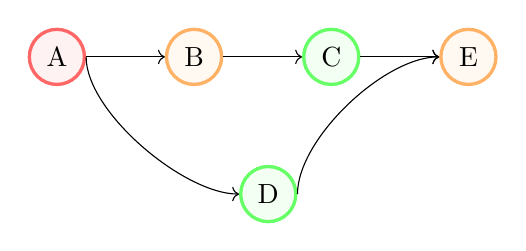
\begin{tikzpicture}
%Nodes
\node[node, red] (node1) {A};
\node[node, orange] (node2) [right=of node1] {B};
\node[node] (node3) [right=of node2] {C};
\node[node] (node4) [below=of node3, xshift=-8mm] {D};
\node[node, orange] (node5) [right=of node3] {E};

%Lines
\draw[->] (node1.east) -- (node2.west);
\draw[->] (node2.east) -- (node3.west);
\draw[->] (node3.east) -- (node5.west);
\draw[->] (node1.east) .. controls +(down:7mm) and +(left:7mm) .. (node4.west);
\draw[->] (node4.east) .. controls +(up:7mm) and +(left:7mm) .. (node5.west);
\end{tikzpicture}
\end{center}

Recall that our traversal heuristic states that we may only consider a node for traversal if all of its in-neighbours have propagated to it. Here, A creates a Promise $P$, propagates its Promise Branches
$p_1$, $p_2$ to B and D, and we see that the number of inputs landed at B equals B's in-degree. We traverse to B.

\begin{center}
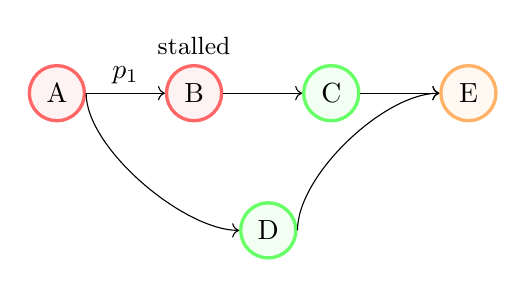
\begin{tikzpicture}
%Nodes
\node[node, red] (node1) {A};
\node[node, red, label={\small stalled}] (node2) [right=of node1] {B};
\node[node] (node3) [right=of node2] {C};
\node[node] (node4) [below=of node3, xshift=-8mm] {D};
\node[node, orange] (node5) [right=of node3] {E};

%Lines
\draw[->] (node1.east) -- (node2.west) node[midway, above] {$p_1$};
\draw[->] (node2.east) -- (node3.west);
\draw[->] (node3.east) -- (node5.west);
\draw[->] (node1.east) .. controls +(down:7mm) and +(left:7mm) .. (node4.west);
\draw[->] (node4.east) .. controls +(up:7mm) and +(left:7mm) .. (node5.west);
\end{tikzpicture}
\end{center}

B is an Arg Node, so the Promise Branch will retrieve its forward output and forward-chain it to obtain the activation at A, then save it to the Promise.
We now stall traversal and enqueue B until the Promise is complete. Our only next option for traversal is D, which has received the other Promise Branch $p_2$ from A as input.

\begin{center}
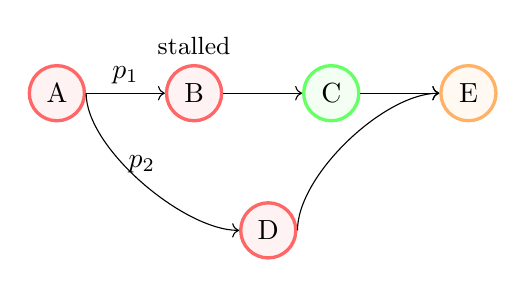
\begin{tikzpicture}
%Nodes
\node[node, red] (node1) {A};
\node[node, red, label={\small stalled}] (node2) [right=of node1] {B};
\node[node] (node3) [right=of node2] {C};
\node[node, red] (node4) [below=of node3, xshift=-8mm] {D};
\node[node, orange] (node5) [right=of node3] {E};

%Lines
\draw[->] (node1.east) -- (node2.west) node[midway, above] {$p_1$};
\draw[->] (node2.east) -- (node3.west);
\draw[->] (node3.east) -- (node5.west);
\draw[->] (node1.east) .. controls +(down:7mm) and +(left:7mm) .. (node4.west) node[midway, above] {$p_2$};
\draw[->] (node4.east) .. controls +(up:7mm) and +(left:7mm) .. (node5.west);
\end{tikzpicture}
\end{center}

We know that now E must be traversed, but see that we never traversed into it from the A->B->C path, so its incoming relevance inputs will never equal its in-degree, and we cannot consider it
for traversal. This creates a circular dependency: C is stalled waiting for A's Promise $P$ to complete, but $P$ cannot complete because its second branch $p_2$ requires accessing E's activation,
and E cannot be visited because it is waiting for C to propagate. The traversal is deadlocked.

The solution, in brief, is to break our traversal heuristic upon such situations, and allow Promise Branches to fully propagate until they reach Arg Nodes.
The specific manner in which this is done is explained fully in Appendix~\ref{appendix:pre-promises}.

A simplified version of the propagation algorithm which considers all these is presented as Algorithm~\ref{alg:promise-propagation}.

Note that this allows delayed computation to occur without the graph traversal pointer having to backtrack or revisit any node not on the current traversal frontier.
Propagation across any given node only occurs once, either directly via tensor relevances or in a delayed manner via Promises. We claim that it follows that the internal nodes recorded
within each Promise's computation path are mutually exclusive among all Promises, though multple Promises may share the same Origin or Arg nodes. We prove this in Appendix~\ref{appendix:unique-chains}.
This allows us to define clear upper bounds on the computational and memory overhead introduced by the Promise system.

\subsection{Theoretical Analysis}
\label{sec:lrp-complexity}

We analyze the computational complexity of our promise-based LRP algorithm in terms of the architectural properties that determine promise resolution requirements.

Let $V_P \subseteq V$ be the set of promise-generating operations in the computation graph $G = (V, E)$.
At the time of writing, the set of promise-generating operations is:
$$V_P = \{v \in V : \text{type}(f_v) \in \{\text{Add}, \text{Sum}, \text{Cat}, \text{Unbind}, \text{Mean}, \text{Stack}\}\}$$
\end{definition}

\begin{definition}[Promise Depth]
For each promise-generating operation $v_p \in V_P$, the Promise Depth is:
$$d(v_p) = \max_{u \in outadj(v_p)} dist(u, argnode)$$
where for every $u$, $argnode$ is its nearest descendent operation that stores a forward activation required by $v_p$.
% The maximum promise depth is:
% $$D = \max_{v_p \in V_P} d(v_p)$$
\end{definition}

\vspace{0.3cm}
\begin{theorem}[Promise-Based LRP Complexity]
Let $G = (V, E)$ be the computation graph of a neural network with $n = |V|$ operations, $m = |E|$ edges, promise-generating set $V_P$, and maximum promise depth $D$.

Let $C_{fwd}, C_{bwd}$ be the most expensive forward and backward pass computation steps, respectively.

Let $S$ be the size of the largest activation cached in the computation graph.

Let $\delta = \sum_{v_p \in V_P} d(v_p)$

Then, the promise-based LRP algorithm has runtime complexity $O((C_{fwd} + C_{bwd}) \cdot (n + m))$, and memory overhead complexity $O(|V_P| \cdot S)$.
% The promise-based LRP algorithm requires $F = 1 + |P| \cdot D$ forward passes and $B = 1$ backward pass, giving total complexity $O((1 + |P| \cdot D) \cdot n + m)$.
\end{theorem}

\begin{proof}
First, we consider that the memory bound is straightforward, as each Promise stores a constant number of tensors representing the \texttt{rout}, \texttt{rins}, and \texttt{args}, and all tensors are bounded above by the largest activation in the model computation.

To prove the time complexity, we analyze the algorithm in three distinct phases:

\textbf{Phase 1 - Initial Forward Pass:} One forward pass is performed to generate the model output and construct the computation graph. This requires $O(C_{fwd} \cdot (n + m))$ time.

\textbf{Phase 2 - Auxiliary Graph Construction:} The algorithm constructs the auxiliary graph $G'$ from the output's computation graph $G$, requiring only graph traversal and no numerical computation. This requires $O(n + m)$ time.

\textbf{Phase 3a - Backward LRP Pass:} The algorithm performs exactly one backward pass through $G'$ to compute relevance propagation. This requires $O(C_{bwd} \cdot (n + m))$ time.

\textbf{Phase 3b - Promise Resolution:} When the LRP traversal encounters a promise-generating operation $v_p \in V_P$ that lacks its required forward activation, a promise object is created. Each promise must traverse backward through the graph until it locates the operation storing its required activation. 

Crucially, our implementation shows that promises never share the same internal nodes in their computation paths. Each promise maintains independent traversal paths (via distinct \texttt{fwd\_list}, \texttt{bwd\_list}, and \texttt{arg\_node\_ind} fields) and resolves separately through individual \texttt{setarg()} calls.
Therefore, each promise requires exactly $d(v_p)$ traversal steps, leading to $d(v_p) \cdot C_{fwd}$ additional forward computations in the worst case, for a total of $\delta = \sum_{v_p \in V_P} d(v_p)$ forward computations when considering all Promises.
Since all computation paths are mutually exclusive, we have that $\delta \leq n$, and so promise resolution overhead has time complexity $O(C_{fwd} \cdot \delta) \in O(C_{fwd} \cdot n)$.

Therefore, the total complexity is in $O((C_{fwd} + C_{bwd}) \cdot (n + m))$, the asymptotic class of a standard backward pass, and memory overhead complexity $O(\delta \cdot S)$, where both $\delta$ and $S$ depend on architectural choices, and $\delta$ is independent of input size.
\end{proof}

\subsubsection{Caching Promise Structures}
\label{sec:promise-caching}
This covers, however, only the first pass of the LRP algorithm. It is worth noting that repeated runs of LRP on the same model architecture yield an identical set of saved Promise computation paths.
As a result, caching these paths can significantly improve the scalability of the algorithm.
Once a Promise's computation path has been defined, it can effectively be reduced to a single node, therefore eliminating the graph traversal overhead of its internal nodes.

Another benefit which arises from both the caching and this reduction is that the traversal order becomes strictly determined by the topological ordering of the nodes.
Recall that due to the issue of Promise Deadlock that can be encountered during initial traversal, propagation of Promises may cause the traversal to temporarily disobey this ordering for the sake of searching ahead for missing activations.
However, if we know the Promise chains beforehand and can reduce them to single nodes, then the order in which we perform computations becomes fully deterministic and independent of edge connections, reducing the graph traversal overhead to $O(n)$.

\section{Experimental Setup}
\label{sec:experiments}
\subsection{Models and Datasets}
To evaluate faithfulness, we used finetuned versions of RoBERTa-large (335M) \cite{liu2019roberta} and Flan-T5-large (780M) \cite{chung2022flant5}
with the SQuAD-v2 question-answering dataset \cite{rajpurkar2018squadv2, chan2021robertasquadv2, lee2023flant5squadv2} for text.
For visual tests, we used the base ViT-b-16 \cite{dosovitskiy2021vit} with the ImageNette-320 \cite{howard2019imagenette} test set and base
VGG16 \cite{simonyan2015vgg} from TorchVision on the CIFAR-10 ImageNet dataset \cite{krizhevsky2009learning}.
The transformer models were all downloaded from HuggingFace. Finetuning settings can be found in respective model cards linked in citations.

\subsection{Evaluating Attributions in Question-Answering Tasks}
We measure the faithfulness of attributions via the accuracy of the top-1 and top-2 attributed tokens being within the answer span predicted
by the model, and the accuracy of the top-1 token being within the span of the ground truth answer. We include also the Intersection-over-Union
(IoU) between the top-2 attributed tokens and the model predicted span. The top-2 accuracy was chosen since QA models produce only two primary
signals for the answer span, not necessarily one for all tokens in the span. We use these top-2 metrics only on with model predictions since
LRP is meant to attribute the model's decision process, not be a predictor of the answer itself. Though, alignment of the top-1 label accuracy
and model exact match rate and F1 score can emphasize explainability strength of the attribution method.
We make use of all answerable examples in the SQuADv2 validation set, and skip examples which the model blatantly predicts incorrectly (when
the start index is after the end index). We run LRP-$\gamma$ with $\gamma_{linear} = 0.001$ for both models, and only enable AttnLRP rules
for the Flan-T5 attributions. See Table~\ref{squadv2-table}

\subsection{Measuring Visual Attribution Faithfulness With Area Between Perturbation Curves}
We measure faithfulness using the Area Between Perturbation Curves (ABPC) \cite{schulz2020abpc, blucher2024pixelflipping}.
We first compute the relevance attributions for each input feature on each example. Then for $n$ iterations, we compute the
Most-Relevant First (MoRF) curve at x = i by masking/occluding the top-i most relevant features from each input sample. We also do this inversely,
masking/occluding the top-i least relevant features from each input sample, to compute the Least-Relevant First (LeRF) curve.
The ABPC is then the difference of their integrals, or $AUC(LeRF) - AUC(MoRF)$.
All image inputs are 3-channel and 224x224 pixels in size. For each step, we occlude 1024 pixels (for the sake of computation time) from each
image by replacing them with their values in a Gaussian-blurred version of the image ($\text{kernel} size=51$, $\sigma=20$). For ViT-b-16, we occlude
the top 4 16x16 patches pooled by max relevance at each step, and for VGG16 we occlude the individual pixels. See Table~\ref{vit-table},
Table~\ref{vgg-table}.

\section{Results}
The text experiments of Table~\ref{squadv2-table} show DynamicLRP attributions to be strong explainers of model behaviour in LLM question answering.
We compare these to the results obtained by Achtibat et al. from LxT (0.94 Top-1 accuracy, 0.84 IoU), though in computing IoU, they consider
hits among the entire ground truth mask, whereas we compare against the model predicted mask and then only its endpoints.
Meanwhile, we see that among all the attribution methods tested in Tables \ref{vit-table} and \ref{vgg-table}, ours and AttnLRP stand among the top of the ABPC metrics. Comprehensiveness is defined
as $AUC(y = baseline) - AUC(MoRF)$ and Sufficiency as $AUC(y = baseline) - AUC(LeRF)$.

\begin{table}[!h]
\begin{center}
  \caption{DynamicLRP Attribution faithfulness measured by top attributed token accuracy against model predictions and labels and IoU with
  predictions with the entire SQuADv2 validation set (5928 examples). EM = Exact Match. Higher is better for all but last two columns.
  Columns marked with (P) are w.r.t. model predictions, (L) are w.r.t. labels. Top-2 accuracy and IoU values in parentheses signify strict
  matching to only the predicted start/end indices, and none of the indices between them. Non-parenthesized values here allow hits on indices
  within the span. All remaining unaccounted examples in the totals were skipped due to exceeding model max token length (512).}
  \label{squadv2-table}
  \begin{tabular}{ lcccccccc }
    \toprule
    \textbf{Model} & \textbf{EM} & \textbf{F1} & \textbf{top-1 (L)} & \textbf{top-1 (P)} & \textbf{top-2 (P)} & \textbf{IoU (P)} & \textbf{Examples} & \textbf{Skipped} \\
    \midrule
    RoBERTa-L & 82.29 & 86.27 & 93.70 & 97.47 & 96.22 (88.95) & 92.70 (80.09) & 5844 & 45 \\
    Flan-T5-L & 83.65 & 90.15 & 95.06 & 98.64 & 94.73 (85.64) & 89.94 (74.86) & 5830 & 36 \\
    \bottomrule
  \end{tabular}
\end{center}
\end{table}

We also demonstrate that DynamicLRP is as faithful than the leading implementation of AttnLRP in the ViT experiment,
and much better than all other alternative methods in every category present, barring the speed of InputXGradient.
In addition, DynamicLRP outperforms the Zennit \cite{anders2021zennit} implementation, SmoothGrad, and Saliency in the VGG evaluations.

\begin{table}[h]
\begin{center}
  \vspace{10pt}
  \caption{ABPC and attribution efficiency metrics for ViT-b-16 experiments. 1000 examples from CIFAR-10 test set.}
  \label{vit-table}
  \begin{tabular}{ lccccc }
    \toprule
    \textbf{Method} & \textbf{ABPC ($\uparrow$)} & \textbf{Comprehensiveness ($\uparrow$)} & \textbf{Sufficiency ($\downarrow$)} & \textbf{Speed (it/s, $\uparrow$)} & \textbf{Peak VRAM ($\downarrow$)} \\
    \midrule
    IG & 0.10 & 0.95 & 0.85 & N/A* & >12GB \\ 
    InputXGrad & -0.0030 & 0.90 & 0.90 & \textbf{59.89} & 2.1GB \\ 
    GradSHAP & 0.074 & 0.94 & 0.87 & 3.32 & 8.6GB \\
    Random & -0.023 & 0.88 & 0.90 & - & - \\
    AttnLRP & \textbf{1.46} & \textbf{1.78} & 0.33 & 6.02 & \textbf{0.96GB} \\
    \midrule
    Ours & \textbf{1.46} & \textbf{1.78} & \textbf{0.32} & 9.74 & 1.6GB \\
    \bottomrule
  \end{tabular}
\end{center}
\vspace{0.1cm}
*N/A in the Speed column signifies that GPU memory limits caused thrashing and prevented the observation of method's true speed.
\vspace{10pt}
\begin{center}
  \caption{ABPC and attribution efficiency metrics for VGG experiments. 3800 examples from ImageNette (320px) validation set.}
  \label{vgg-table}
  \begin{tabular}{ lccccc }
    \toprule
    \textbf{Method} & \textbf{ABPC ($\uparrow$)} & \textbf{Comprehensiveness ($\uparrow$)} & \textbf{Sufficiency ($\downarrow$)} & \textbf{Speed (it/s, $\uparrow$)} & \textbf{Peak VRAM ($\downarrow$)} \\
    \midrule
    Saliency & 0.73 & 2.58 & 1.85 & \textbf{156.83} & \textbf{0.89GB} \\ 
    SmoothGrad & 1.50 & \textbf{2.87} & 1.37 & 8.90 & 0.90GB \\ 
    Random & -0.0022 & 2.40 & 2.40 & - & - \\
    Zennit LRP & 1.69 & 2.72 & 1.02 & 29.41 & 1.4GB \\
    \midrule
    Ours & \textbf{1.77} & 2.65 & \textbf{0.88} & 21.79 & 2.3GB \\
    \bottomrule
  \end{tabular}
\end{center}
\end{table}

What we also demonstrate is the framework's capability to adopt rules defined by other implementations. In the ViT experiment, we tuned our LRP to behave similarly to specifications defined in AttnLRP \cite{achtibat2024attnlrp},
using $\gamma$-LRP for Convolutional and Linear layers ($\gamma_{conv} = 130$, $\gamma_{linear} = 0.001$), while routing relevance only through the final matrix multiplication of Attention modules and skipping the softmax.

\subsection{Architecture-Specific Factors on LRP Performance}

\begin{definition}[Promise Density]
The promise density of a neural network architecture is defined as:
$$\rho = \frac{|V_P|}{|V|}$$
where $|V_P|$ is the number of promise-generating operations and $|V|$ is the total number of operations in the computation graph.
\end{definition}

We present in Table~\ref{architecture-promises-table} the $d_{model}$, model depth, number of Promises, number of internal nodes in Promise paths, average Promise path
length, Promise Density, and number of autograd nodes specific to each tested architecture.

\begin{table}[!h]
\begin{center}
  \caption{Architecture-specific values relating to the Promise System's impact on LRP efficiency. We include a separate row for the
  (F)ine(T)uned version of Flan-T5-large which uses LoRA adapters, changing some of these values drastically.
  Depth is in terms of either number of (T)ransformer layers or (C)onvolutional layers.}
  \label{architecture-promises-table}
  \begin{tabular}{ lccccccc  }
    \toprule
    \textbf{Model} & \textbf{$d_{model}$} & \textbf{Depth} & \textbf{Promises} & \textbf{Internal nodes} & \textbf{$\delta$} & \textbf{$\rho$} & \textbf{Total nodes} \\
    \midrule
    RoBERTa-large & 1024 & 24 (T) & 243 & 48 & 438 & 0.166 & 1,465 \\ 
    Flan-T5-large & 1024 & 48 (T) & 798 & 348 & 980 & 0.140 & 5,713 \\ 
    Flan-T5-large (FT) & 1024 & 50 (T) & 847 & 1,524 & 2,972 & 0.0777 & 10,897 \\ 
    ViT-b-16 & 768 & 1 (C) 12 (T) & 224 & 27 & 227 & 0.288 & 779 \\ 
    VGG16 & 512 & 13 (C) & 32 & 0 & 32 & 0.356 & 90 \\ 
    \bottomrule
  \end{tabular}
\end{center}
\end{table}

\section{Discussion}
The recorded values from Table~\ref{architecture-promises-table} provide insight on how the Promise System affects runtime and provide
empirical $|V_P|$ and $\delta$ to help reason about the theoretical memory and runtime complexities.
The most striking observation comes from the difference in $\rho$ between the two versions of Flan-T5-large. While the finetuned T5 has
nearly twice as many autograd nodes and much higher $\delta$, the number of Promises does not increase by nearly the same scale.

The memory improvement of AttnLRP over our LRP is likely due to the fact that it does not require the full autograd
computation graph to be stored, only the subgraphs associated with the above mentioned layers/modules, as well as activations
and normalization layers. This is characteristic to the implementation, which is built on the Zennit library \cite{anders2021zennit}.
Any additional operations performed do not have autograd nodes saved, and thus reduce total peak VRAM usage, as opposed to our method which tracks such operations.

\subsection{Operation Coverage}

By breaking LRP down to the level of tensor operations, we knowingly take on the task of covering a sufficiently large portion of the operation space to make this useful across a wide range of models.
However, consider that the set of tensor operations we are interested in, specifically mathematical and shape operations, is a bounded and well-defined set. 
This places a tangible and conceptual limit on our implementation scope.

There are also case-by-case implementation considerations.
In shape operations, which manipulate only the structure of tensors, the task of relevance propagation reduces to accumulating relevance at the
inputs which map to the output. Here, we simply reuse the functions from gradient backpropagation, which do exactly this and are produced by the auto-differentiation library.
Activation functions such as ReLU, GELU, etc. have been shown to correspond to Identity propagation functions, requiring no implementation overhead.
Finally, fused/composite operations can re-routed or decomposed during auxiliary graph construction (Algorithm \ref{alg:graph-construction}) into
components we already handle.

\begin{table}[!h]
\begin{center}
  \caption{DynamicLRP operation coverage breakdown of 15 models spanning vision, text, and audio modalities. \textbf{Unique Ops} indicates the number of distinct operation types in each model's computation graph.}
  \label{coverage-table}
  \begin{tabular}{ lcccc }
    \toprule
    \textbf{Model} & \textbf{Modality} & \textbf{Covered Nodes} & \textbf{Unique Ops covered} \\
    \midrule
    VGG16 \cite{simonyan2015vgg} & Vision & 90/90 & 9/9 \\
    ResNet-50 \cite{he2015resnet} & Vision & 339/339 & 10/10 \\
    ViT-b-16 \cite{dosovitskiy2021vit} & Vision & 779/779 & 16/16 \\
    EfficientNetv2-medium \cite{tan2021efficientnetv2} & Vision & 1,526/1,526 & 12/12 \\
    SigLIP-2-So400m-base14-384 \cite{tschannen2025siglip2} & Vision & 2,178/2,178 & 19/19 \\
    Wav2Vec2-xls-r-300m \cite{babu2021xlsr} & Audio & 2,021/2,022 & 18/19 \\
    whisper-small \cite{radford2022whisper} & Audio & 2,729/2,729 & 22/22 \\
    GPT-2 \cite{radford2019gpt2} & Language & 885/885 & 19/19 \\
    RoBERTa-large \cite{liu2019roberta} & Language & 1,461/1,461 & 14/14 \\
    Llama3.2-1B \cite{dubey2024llama3} & Language & 1,787/1,787 & 24/24 \\
    Gemma-3-270m-it \cite{gemmateam2025gemma3} & Language & 2,482/2,482 & 24/24 \\
    Qwen3-0.6B \cite{yang2025qwen3} & Language & 2,590/2,590 & 18/18 \\
    Flan-T5-large \cite{chung2022flant5} & Language & 5,713/5,713 & 24/24 \\
    DePlot \cite{liu2022deplot} & Vision/Language & 2,863/2,863 & 23/23 \\
    Mamba-130m \cite{gu2024mamba} & State Space & 3,397/3,421 & 25/26 \\
    \midrule
    \textbf{Aggregate} & - & \textbf{31,440/31,465} & - \\
    \bottomrule
  \end{tabular}
  \vspace{5pt}
  \caption{Uncovered operation breakdown, where applicable.}
  \begin{tabular}{| c | c  c |}
    \hline
    {Model} & {Uncovered Ops} & {Node count} \\
    \hline
    Wav2Vec2-xls-r-300m & WeightNormInterface & 1 \\
    \hline
    Mamba-130m & SplitWithSize & 24 \\
    \hline
  \end{tabular}
\end{center}
\end{table}

We validated model-agnostic coverage by analyzing computation graphs from 15 diverse architectures spanning vision (CNNs, ViTs), language (GPT, BERT, T5, Llama), audio
(Wav2Vec2, Whisper), multimodal (DePlot), and state-space models (Mamba). As shown in Table~\ref{coverage-table}, our implementation achieved \textbf{99.92\% node coverage
(31,440/31,465 nodes)} across all architectures \textbf{without any model-specific code modifications}. The 25 uncovered nodes (0.08\%) correspond to two operations:
\texttt{WeightNormInterface} (weight normalization utility, 1 node) and \texttt{SplitWithSize} (variant of \texttt{Split}, 24 nodes). Both could be trivially
supported by extending existing rules. We see that despite increasing model sizes and diversity, modern architectures are composed of only a small set of operations.

\subsection{Extensibility to Other Deep Learning Frameworks}
While it may seem that this design is strictly PyTorch-specific, we claim that the Promise-based Dynamic LRP can be extended to any deep learning
framework with an auto-differentiation library.

We consider that differentiation is first and foremost a mathematical concept, and auto-differentiation stricly relies on computation graphs.
This implies two important invariants across any auto-differentiation engine.
Being built on computation graphs, these engines themselves are defined at the operation level, and for any function to be differentiated, the set of givens required
is purely characteristic to the mathematical properties of the function in question, not the framework or programming language being used.

Thus, all implementations of auto-differentiation will be required to store the same minimum set of data for each function they share, in
the structure of a computation graph.
This signifies to us that the concept of operation-level LRP is sound and viable in any such deep-learning framework.

The Promise System allows even further flexibility to this, as its core purpose is the retrieval of forward pass activations not found in
the computation graph during the backward pass. Therefore, any differences between frameworks in the backward context caching will also
be overcome by our framework.

\bibliography{main}
\iftoggle{arxiv}{
  % arXiv references in a generic style, or ICLR style
  \bibliographystyle{iclr2025_conference}
}{
  % bst style for the journal/conference version goes here
  % For NeurIPS there is no house bst file; you can use ICLR bst instead
  % \bibliographystyle{iclr2025_conference}
}

\newpage

\appendix
\section{List of Covered Operations}
\label{appendix:covered-operations}
Below is the list of currently supported operations for DynamicLRP.
\begin{table}[!h]
\begin{center}
  \begin{tabular}{ll}
    \toprule
    \textbf{Category} & \textbf{Operations} \\
    \midrule
    \textbf{Arithmetic} & Add, Sub, Mul, Div, Neg, Sqrt, Rsqrt, Pow, Exp, Log \\
    \textbf{Linear Algebra} & Mm, Bmm, Convolution \\
    \textbf{Aggregation} & Sum, Mean, Cat, Stack, Unbind, Split, Max, Gather \\
    \textbf{Shape Manipulation} & View, Reshape, Transpose, Permute, Expand, Repeat, Squeeze, Unsqueeze \\
    \textbf{Indexing and Selection} & Slice, Index, Select \\
    \textbf{Pooling} & MaxPool2D, MaxPool3D, AdaptiveAvgPool2D \\
    \textbf{Normalization} & NativeLayerNorm, NativeBatchNorm \\
    \textbf{Attention} & SDPA \\
    \textbf{Activations} & GELU, SiLU, ReLU, Softmax \\
    \textbf{Other} & MaskedFill, Clone, ToCopy, NativeDropout, Embedding \\
    \bottomrule
  \end{tabular}
\end{center}
\end{table}

\section{Algorithms}
\begin{algorithm}[H]
  \caption{Computation Graph Construction}
  \label{alg:graph-construction}
  \begin{algorithmic}[1]
    \Require Model output $hidden\_states$
    \Ensure In-adjacency list $in\_adj$, Out-adjacency list $out\_adj$, Topologically sorted nodes $topo\_stack$
    \State Initialize $in\_adj \gets \emptyset$, $out\_adj \gets \emptyset$
    \State Initialize $visited \gets \emptyset$, $topo\_stack \gets \emptyset$
    \State $root \gets hidden\_states.grad\_fn$
    \State \Call{DFS}{$root$, $in\_adj$, $out\_adj$, $visited$, $topo\_stack$}
    \Return $in\_adj$, $out\_adj$, $topo\_stack$
    \Function{DFS}{$fcn$, $in\_adj$, $out\_adj$, $visited$, $topo\_stack$}
      \If{$fcn = \text{None}$ or $fcn \in visited$}
        \State \Return
      \EndIf
      \State $visited \gets visited \cup \{fcn\}$
      \For{each $child \in fcn.next\_functions$}
        \State $out\_adj[fcn].append(child)$
        \State $in\_adj[child].append(fcn)$
        \State \Call{DFS}{$child$, $in\_adj$, $out\_adj$, $visited$, $topo\_stack$}
      \EndFor
      \State $topo\_stack.push(fcn)$
    \EndFunction
  \end{algorithmic}
\end{algorithm}

\begin{algorithm}[H]
  \caption{Operation-Level Relevance Propagation With Promises}
  \label{alg:promise-propagation}
  \begin{algorithmic}[1]
    \Require Model output $hidden\_states$, Relevance interpretation target $target\_node$, Auxiliary graph $in\_adj$, $out\_adj$, Output relevance $R_{out}$
    \Ensure Input relevance $R_{in}$
    \State Initialize as in Algorithm 2

    \While{$stack$}
      \State $curnode \gets stack.pop()$
      \State $curnode\_in\_rel = node\_inputs[curnode]$
      \If{$curnode == target\_node$}
        \Return $R_{in} := curnode\_in\_rel$
      \ElsIf{$curnode$ requires Promise}
        \State $curnode.promise \gets create\_new\_promise(type(curnode), R_{out})$
        \State $curnode\_outputs \gets curnode.promise.branches$
      \Else
        \State $prop\_fcn \gets fcn\_map[type(curnode)]$
        \State $curnode\_outputs \gets prop\_fcn(curnode\_in\_rel)$
      \EndIf
      \For{each $child, output \in zip(out\_adj[curnode], curnode\_outputs)$}
        \State $node\_inputs[child].add(output)$
        \State $nodes\_pending[child] \gets nodes\_pending[child] - 1$
        \If{$nodes\_pending[child] == 0$}
          \State $stack.push(child)$
        \EndIf
      \EndFor
    \EndWhile
  \end{algorithmic}
\end{algorithm}

We extend the standard propagation functions to handle Promise inputs. Depending on whether the current node is an
Arg Node, the function either records the chain or resolves and completes the Promise.

\begin{algorithm}[H]
  \caption{Non-Arg Node Propagation Function Promise Handling}
  \label{alg:non-argnode-propagation}
  \begin{algorithmic}[1]
    \Require Autograd Node $node$, Propagation input $R_{out}$
    \Ensure Propagation output list $R_{in}$

    \If{$R_{out}$ is a Promise Branch}
      \State Define $fwd$ as a closure of $node$'s forward pass.
      \State Define $bwd$ as a closure of $node$'s relevance distribution logic.
      \State $R_{out}.record(fwd, bwd)$
      \Return $R_{out}$
    \EndIf

    \State \textit{// Propagate $R_{out}$...}
    \Return $R_{in}$
  \end{algorithmic}
\end{algorithm}

\begin{algorithm}[H]
  \caption{Arg Node Propagation Function Promise Handling}
  \label{alg:argnode-propagation}
  \begin{algorithmic}[1]
    \Require Autograd Node $node$, Propagation input $R_{out}$
    \Ensure Propagation output list $R_{in}$

    \If{$R_{out}$ is a Promise Branch}
      \State Define $retrieve\_fwd\_output$ as a function that extracts $node$'s forward pass output given its saved tensors.
      \State $activation = retrieve\_fwd\_output(node)$
      \State $R_{out}.set\_arg(activation)$
      \State $R_{out}.trigger\_promise\_completion()$
      \If{$R_{out}.promise\_is\_complete$}
        $R_{out} = R_{out}.propagated\_relevance$
      \Else
        \State \textit{// Signal for queueing this Node until the Promise is complete}
        \Return
      \EndIf
    \EndIf

    \State \textit{// Propagate $R_{out}$...}
    \Return $R_{in}$
  \end{algorithmic}
\end{algorithm}

\section{Implementation Details}
Our implementation uses PyTorch hooks to record operations during the forward pass and constructs the computation graph dynamically. Each operation creates a promise object, which stores the propagation rule and tracks readiness and completeness.

\textbf{Python Example: Promise System}
Below is a simplified Python pseudocode that captures the core logic of the Promise System:

\begin{verbatim}

class PromiseBranch:
  def __init__(self, promise_obj, index):
    self.promise = promise_obj
    self.promise_dict = promise.metadata_dict
    self.index = index
    self.fwd_chain = []
    self.bwd_chain = []
    self.children = [] # Recall that the child connection is from Branch -> Promise

  def record_fwd(self, fwd_closure):
    self.fwd_chain.append(fwd_closure)

  def record_bwd(self, bwd_closure):
    self.bwd_chain.append(bwd_closure)

  def setarg(self, val):
    # Brings args from the Arg Node to the Origin Node
    # Assumes that fwd_chain has recorded all node fwd closures leading up to an Arg Node
    for fcn in self.fwd_chain:
      # Iteratively apply the forward chain operations
      val = fcn(val)
    self.promise_dict["args"][self.index] = val

    self.promise_dict["ready"] = all(arg is not None for arg in self.promise_dict["args"])
    if self.promise_dict["ready"]:
      self.promise.trigger_completion()

  def exec_bwd(self, val):
    # Brings relevances from the Origin Node to the Arg Node
    # Assumes that bwd_chain has recorded all node bwd closures leading up to an Arg Node
    for fcn in reverse(self.bwd_chain):
      # Iteratively apply the backward chain operations in reverse order from what they were recorded in
      val = fcn(val)
    self.promise_dict["rins"][self.index] = val

class Promise:
  def __init__(self, output_relevance, op, num_branches, parent_promises)
    self.op = op
    self.parents = parent_promises # And the parent connection is from Promise -> Branch
    self.metadata_dict = {
      "rout": output_relevance,
      "ready": False,
      "complete": False,
      "args": [None] * num_branches,
      "rins": [None] * num_branches,
    }

    # metadata_dict is mutable, so all branches can write to it as a shared location,
    #  using their respective index
    self.branches = [ PromiseBranch(self, i) for i in range(num_branches) ]
  
  def accumulate_rout(self, val):
    # May be overridden based on the Promise operation type, but this is a general default for simplicity
    self.metadata_dict["rout"] += val

  def trigger_completion(self):
    if len(pending_parents := list(filter(lambda parent: not parent.complete, self.parents))):
      # If Promise has any parent Promise Branches that have not been completed yet, try to trigger them by
      #  setting their args with this Promise's op result
      # This potentially sets off a mutual recursion loop between PromiseBranch.setarg() and
      #  Promise.trigger_completion() calls.
      for parent in pending_parents:
        parent.setarg(self.op(*self.metadata_dict["args"]))
    else:
      # Otherwise, we can proceed with relevance backprop
      # Custom propagation rule for each operation type
      self.relevance = propagate_relevance(type(self.op), output_relevance, self.metadata_dict["args"])
      for i, branch in enumerate(self.branches):
        # Propagates the distributed relevances from Origin Node back to each end-of-Branch Arg Node
        branch.exec_bwd(self.relevance[i])
        for child in branch.children:
          # self.metadata_dict["rins"][i] is updated within branch.exec_bwd()
          child.accumulate_rout(self.metadata_dict["rins"][i])
      self.metadata_dict["complete"] = True

      # Recurse
      for branch in self.branches:
        for child in branch.children:
          child.trigger_completion()

\end{verbatim}

\textbf{Explicit Steps in the Algorithm}
\begin{enumerate}
  \item \textbf{Forward Pass:} Get the model output and computation graph built by the auto-differentiation library.
  \item \textbf{Graph Augmentation Pass:} Attach any additional required metadata for LRP to each node in the computation graph. This includes in-neighbours, topological ordering, and computation flags. See Algorithm~\ref{alg:graph-construction}.
  \item \textbf{Backward Pass:} Starting from the output, traverse the graph using the Traversal Heuristic (Def~\ref{def:traversal-heuristic}). A node is traversed when all output relevance is received, or when it is part of a Promise's resolution path, and marked as propagated when it distributes relevance to its inputs.
  \item \textbf{Relevance Aggregation:} Input nodes collect relevance from all incoming promises, yielding the final attribution scores.
\end{enumerate}

\textbf{Readiness and Completeness}
\begin{itemize}
  \item \textbf{Readiness:} A promise is ready when all output relevance (from downstream nodes) has been received.
  \item \textbf{Completeness:} A promise is complete when it has distributed its relevance to all inputs according to its propagation rule.
\end{itemize}

This mechanism ensures that relevance is propagated in accordance with the mathematical definition of LRP, maintaining conservation and proportionality at each node.

\section{Promise Examples}
\subsection{Basic Promise Mechanism}
\label{appendix:basic-promise-example}
Consider the following subgraph in a computation graph. Suppose nodes A, B, C, D are all nodes which do not store
any forward activations, and E is one which does and allows us to retrieve or recompute its forward pass output.
Furthermore, suppose that node A is one which requires some forward activation to compute relevance propagation,
and nodes B, C, D are all operations whose backward relevance propagations do not require any forward activations.

\vspace{0.7cm}
\begin{center}
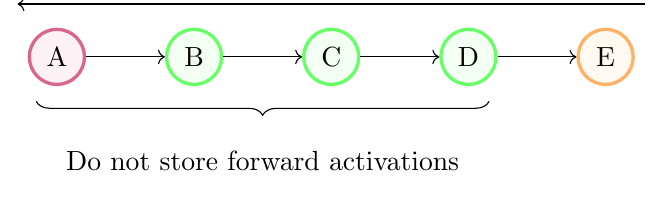
\begin{tikzpicture}
  \node[node, purple] (node1) {A};
  \node[node] (node2) [right=of node1] {B};
  \node[node] (node3) [right=of node2] {C};
  \node[node] (node4) [right=of node3] {D};
  \node[node, orange] (node5) [right=of node4] {E};

  \draw[->] (node1.east) -- (node2.west);
  \draw[->] (node2.east) -- (node3.west);
  \draw[->] (node3.east) -- (node4.west);
  \draw[->] (node4.east) -- (node5.west);
  \begin{scope}[transform canvas={yshift=.3cm}]
    \draw[->, shorten <= -0.5cm, shorten >= -0.5cm] (node5.north) -- (node1.north) node[midway, above] {Model forward};
  \end{scope}
  \draw [decorate,decoration={brace,amplitude=5pt,mirror,raise=2ex}]
    (node1.south west) -- (node4.south east) node[midway,yshift=-3em]{Do not store forward activations};
\end{tikzpicture}
\end{center}
\vspace{0.3cm}

Thus, node A is the limiting factor here. Without this forward activation it requires, we cannot continue relevance
propagation. But we know there is some node further down the traversal which saves some forward activation(s),
and if we traverse to it, we will also know all the operations between it and node A, giving us a way to reconstruct
the activation at node A (see Proposition below).

\textbf{Proposition 1:} For any node $v$ in a computation graph, there exists at least one node descendent to $v$
which stores a forward activation, which we call an Arg Node.

\begin{proof}
  We prove this using the programming paradigm of PyTorch. We have that every model output is a function of the
  model inputs and parameters. By the nature of backpropagation, we must compute the gradients of the loss w.r.t.
  each parameter, but we require the values of the parameters at each layer to compute the gradients w.r.t. the
  parameters at the preceding layer.
  
  Since every part of the model is a function of the inputs and parameters in some way, their nodes in the
  computation graph must have out-degree 0. Therefore, as long as the model inputs are set to track gradients,
  every sink node of the DAG will contain a parameter or input, which are forward activations.
  
  If any node did not eventually lead to such a sink node, that would imply that none of the nodes along this
  path require gradient tracking. But then this path should not exist in the computation graph at all.

  So, all other nodes in the computation graph must be ancestors of some such sink node, and this statement holds true.
\end{proof}

Now, for each node $v$, consider $fwd_v$ to be a closure of the node's forward operation, and $bwd_v$ to be a closure of
its backward relevance propagation function.

Let $y_E$ be the forward output at node E. Then, we can reconstruct the forward input at node A, $x_A$, by computing
$x_A = fwd_B(fwd_C(fwd_D(y_E)))$.

Let $R_A$ be the accumulated relevance at A from its in-neighbours. When we have recomputed $x_A$, we can then compute
$R_{B \leftarrow A} = bwd_A(R_A, x_A)$. And similarly, we compute $R_{E \leftarrow D} = bwd_D(bwd_C(bwd_B(R_{B \leftarrow A})))$.

We accomplish this during traversal with the use of Promises, enabling a lazy evaluation of these values. We colour nodes red upon
traversing them. We also indicate the location of the traversal pointer with $\uparrow$.

\begin{center}
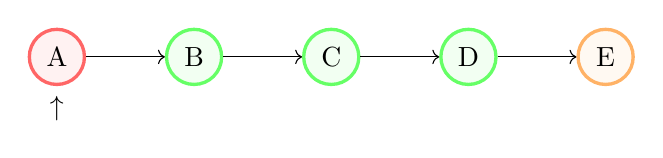
\begin{tikzpicture}
  \node[node, red, label=below:{$\uparrow$}] (node1) {A};
  \node[node] (node2) [right=of node1] {B};
  \node[node] (node3) [right=of node2] {C};
  \node[node] (node4) [right=of node3] {D};
  \node[node, orange] (node5) [right=of node4] {E};

  \draw[->] (node1.east) -- (node2.west);
  \draw[->] (node2.east) -- (node3.west);
  \draw[->] (node3.east) -- (node4.west);
  \draw[->] (node4.east) -- (node5.west);
\end{tikzpicture}
\end{center}

We encounter node A, which we find requires a Promise. We instantiate the Promise metadata object $P$ and propagate its Branch $b_P$ to its out-neighbour, and continue traversal.

\begin{center}
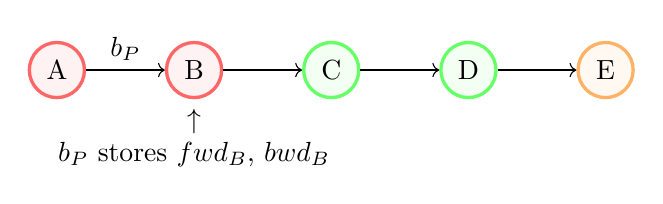
\begin{tikzpicture}
  \node[node, red] (node1) {A};
  \node[node, red] (node2) [right=of node1] {B};
  \node[align=center,anchor=north] (lab) at (node2.south) {$\uparrow$\\$b_P$ stores $fwd_B$, $bwd_B$};
  \node[node] (node3) [right=of node2] {C};
  \node[node] (node4) [right=of node3] {D};
  \node[node, orange] (node5) [right=of node4] {E};

  \draw[->] (node1.east) -- (node2.west) node[midway, above] {$b_P$};
  \draw[->] (node2.east) -- (node3.west);
  \draw[->] (node3.east) -- (node4.west);
  \draw[->] (node4.east) -- (node5.west);
\end{tikzpicture}
\end{center}

Upon reaching node B, since it is not an Arg Node, $b_P$ will record $fwd_B$ and $bwd_B$, then will be passed on to B's out-neighbour.
It will continue and do this for C and D.

\begin{center}
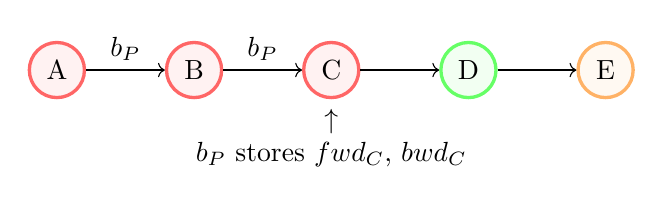
\begin{tikzpicture}
  \node[node, red] (node1) {A};
  \node[node, red] (node2) [right=of node1] {B};
  \node[node, red] (node3) [right=of node2] {C};
  \node[align=center,anchor=north] (lab) at (node3.south) {$\uparrow$\\$b_P$ stores $fwd_C$, $bwd_C$};
  \node[node] (node4) [right=of node3] {D};
  \node[node, orange] (node5) [right=of node4] {E};

  \draw[->] (node1.east) -- (node2.west) node[midway, above] {$b_P$};
  \draw[->] (node2.east) -- (node3.west) node[midway, above] {$b_P$};
  \draw[->] (node3.east) -- (node4.west);
  \draw[->] (node4.east) -- (node5.west);
\end{tikzpicture}
\end{center}

\begin{center}
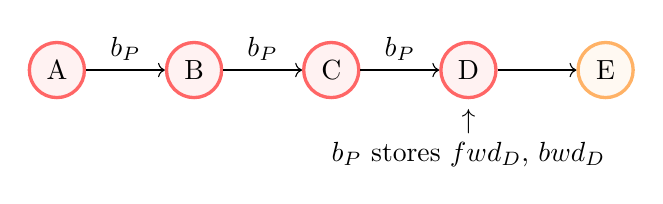
\begin{tikzpicture}
  \node[node, red] (node1) {A};
  \node[node, red] (node2) [right=of node1] {B};
  \node[node, red] (node3) [right=of node2] {C};
  \node[node, red] (node4) [right=of node3] {D};
  \node[align=center,anchor=north] (lab) at (node4.south) {$\uparrow$\\$b_P$ stores $fwd_D$, $bwd_D$};
  \node[node, orange] (node5) [right=of node4] {E};

  \draw[->] (node1.east) -- (node2.west) node[midway, above] {$b_P$};
  \draw[->] (node2.east) -- (node3.west) node[midway, above] {$b_P$};
  \draw[->] (node3.east) -- (node4.west) node[midway, above] {$b_P$};
  \draw[->] (node4.east) -- (node5.west);
\end{tikzpicture}
\end{center}

Until, finally, $b_P$ encounters node E, which is an Arg Node, and we are able to retrieve the forward pass output of E, $y_E$.

\begin{center}
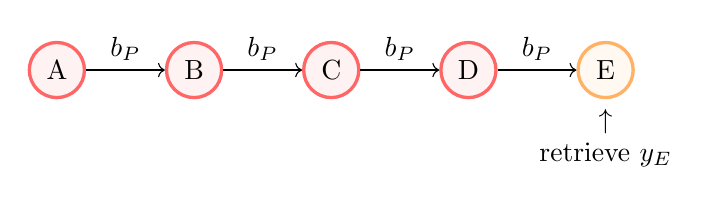
\begin{tikzpicture}
  \node[node, red] (node1) {A};
  \node[node, red] (node2) [right=of node1] {B};
  \node[node, red] (node3) [right=of node2] {C};
  \node[node, red] (node4) [right=of node3] {D};
  \node[node, orange] (node5) [right=of node4] {E};
  \node[align=center,anchor=north] (lab) at (node5.south) {$\uparrow$\\retrieve $y_E$};

  \draw[->] (node1.east) -- (node2.west) node[midway, above] {$b_P$};
  \draw[->] (node2.east) -- (node3.west) node[midway, above] {$b_P$};
  \draw[->] (node3.east) -- (node4.west) node[midway, above] {$b_P$};
  \draw[->] (node4.east) -- (node5.west) node[midway, above] {$b_P$};
\end{tikzpicture}
\end{center}

We then:
\begin{itemize}
  \item Use the stored $fwd$ closures from B, C, D to compute $x_A = fwd_B(fwd_C(fwd_D(y_E)))$, and store it within the Promise metadata object $P$.
  \item Check in $P$ if the Promise is now in Ready state (all branches have found an Arg Node), in this case there is only the one branch.
  \item If Ready, and the Promise has no incomplete parent Promises (explained the next section), compute $R_{E \leftarrow A} = bwd_D(bwd_C(bwd_B(bwd_A(R_A, x_A))))$.
\end{itemize}

\vspace{0.7cm}
\begin{center}
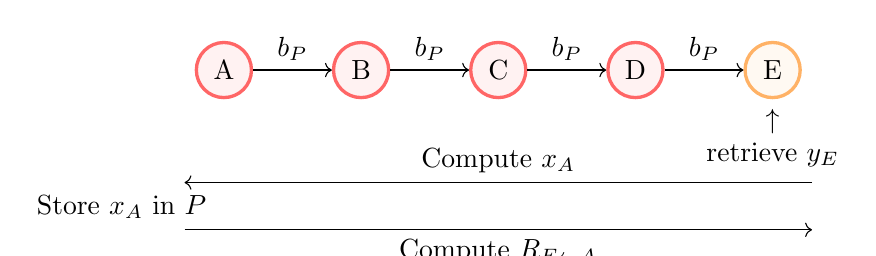
\begin{tikzpicture}
  \node[node, red] (node1) {A};
  \node[node, red] (node2) [right=of node1] {B};
  \node[node, red] (node3) [right=of node2] {C};
  \node[node, red] (node4) [right=of node3] {D};
  \node[node, orange] (node5) [right=of node4] {E};
  \node[align=center,anchor=north] (lab) at (node5.south) {$\uparrow$\\retrieve $y_E$};
  \node[align=center,anchor=north, yshift=-1.1cm, xshift=-1.3cm] (label1) at (node1.south) {Store $x_A$ in $P$};

  \draw[->] (node1.east) -- (node2.west) node[midway, above] {$b_P$};
  \draw[->] (node2.east) -- (node3.west) node[midway, above] {$b_P$};
  \draw[->] (node3.east) -- (node4.west) node[midway, above] {$b_P$};
  \draw[->] (node4.east) -- (node5.west) node[midway, above] {$b_P$};
  \begin{scope}[transform canvas={yshift=-1.8cm}]
    \draw[->, shorten <= -0.5cm, shorten >= -0.5cm] (node5.north) -- (node1.north) node[midway, above] {Compute $x_A$};
  \end{scope}
  \begin{scope}[transform canvas={yshift=-2.4cm}]
    \draw[->, shorten <= -0.5cm, shorten >= -0.5cm] (node1.north) -- (node5.north) node[midway, below] {Compute $R_{E \leftarrow A}$};
  \end{scope}
\end{tikzpicture}
\end{center}
\vspace{0.3cm}

And now, we have lazily computed the propagations of the path starting from A and ending at E, while keeping the traversal pointer from
backtracking any previously visited nodes. Blue indicates relevance propagation is complete at that node.

\begin{center}
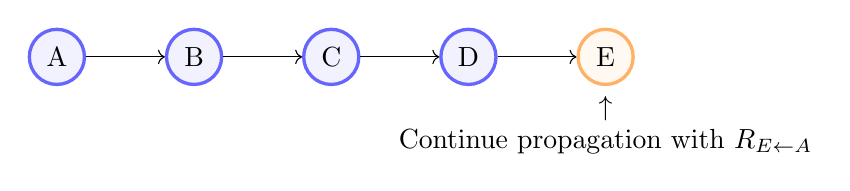
\begin{tikzpicture}
  \node[node, blue] (node1) {A};
  \node[node, blue] (node2) [right=of node1] {B};
  \node[node, blue] (node3) [right=of node2] {C};
  \node[node, blue] (node4) [right=of node3] {D};
  \node[node, orange] (node5) [right=of node4] {E};
  \node[align=center,anchor=north] (lab) at (node5.south) {$\uparrow$\\Continue propagation with $R_{E \leftarrow A}$};

  \draw[->] (node1.east) -- (node2.west);
  \draw[->] (node2.east) -- (node3.west);
  \draw[->] (node3.east) -- (node4.west);
  \draw[->] (node4.east) -- (node5.west);
\end{tikzpicture}
\end{center}

\subsection{Promise Trees and Resolution}
\label{appendix:promise-trees}
A Promise Tree is created when a promise-generating operation receives a Promise as relevance input.
The new Promise specific to that operation is created and linked to the input Promise with parent-child connections.

In this example, A and B are promise-generating operations, marked purple, and D, E, C are Arg Nodes, marked orange.

We also use "->" to indicate the node at which the traversal pointer is pointing at each step.

\begin{center}
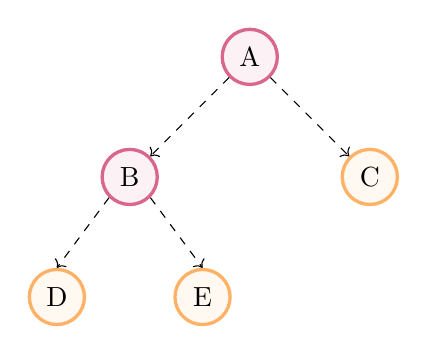
\begin{tikzpicture}
  \node[node, purple] (node1) {A};
  \node[node, purple] (node2) [below left=of node1] {B};
  \node[node, orange] (node3) [below right=of node1] {C};
  \node[node, orange] (node4) [below left=of node2, xshift=0.6cm] {D};
  \node[node, orange] (node5) [below right=of node2, xshift=-0.6cm] {E};

  \draw[dashed, ->] (node1.south west) -- (node2.north east);
  \draw[dashed, ->] (node1.south east) -- (node3.north west);
  \draw[dashed, ->] (node2.south west) -- (node4.north);
  \draw[dashed, ->] (node2.south east) -- (node5.north);

\end{tikzpicture}
\end{center}

We mark nodes as red when we have traversed them, blue when we have propagated relevance through them.
It is important to note the difference between these two states due to the delaying of propagation through Promises.
Node A is traversed first, and propagates Promise Branches $b_{A,1}$ and $b_{A,2}$ through to its out-neighbours.

\begin{minipage}{.5\textwidth}
\begin{center}

\vspace{0.3cm}
Computation Graph

\vspace{0.3cm}
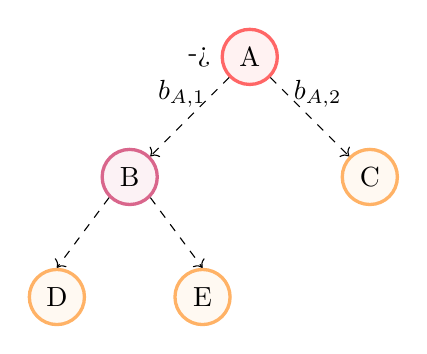
\begin{tikzpicture}
  \node[node, red, label=left:{->}] (node1) {A};
  \node[node, purple] (node2) [below left=of node1] {B};
  \node[node, orange] (node3) [below right=of node1] {C};
  \node[node, orange] (node4) [below left=of node2, xshift=0.6cm] {D};
  \node[node, orange] (node5) [below right=of node2, xshift=-0.6cm] {E};

  \draw[dashed, ->] (node1.south west) -- (node2.north east) node[midway, above, xshift=-0.1cm] {$b_{A,1}$};
  \draw[dashed, ->] (node1.south east) -- (node3.north west) node[midway, above, xshift=0.1cm] {$b_{A,2}$};
  \draw[dashed, ->] (node2.south west) -- (node4.north);
  \draw[dashed, ->] (node2.south east) -- (node5.north);

\end{tikzpicture}
\end{center}
\end{minipage}
\begin{minipage}{.5\textwidth}
\begin{center}

\vspace{0.3cm}
Promise Tree

\vspace{0.3cm}
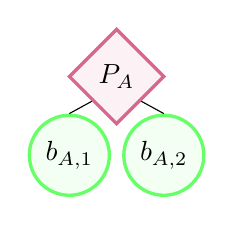
\begin{tikzpicture}
  \node[diamondnode, purple] (node1) {$P_A$};
  \node[node] (node2) [yshift=-1.0cm, xshift=-0.6cm] {$b_{A,1}$};
  \node[node] (node3) [yshift=-1.0cm, xshift=0.6cm] {$b_{A,2}$};

  \draw (node1.south west) -- (node2.north);
  \draw (node1.south east) -- (node3.north);
\end{tikzpicture}
\end{center}
\end{minipage}

We traverse to node B now, and find that it receives Promise Branch $b_{A,1}$. But B is a promise-generating operation, so a new Promise $P_B$ is created.
$P_B$ is added as a child of the branch $b_{A,1}$ and $b_{A,1}$ is added as a parent to $P_B$, creating a Promise Tree. B then propagates the branches of $P_B$, $b_{B,1}$ and $b_{B,2}$ to its out-neighbours.

\begin{minipage}{.5\textwidth}
\begin{center}

\vspace{0.3cm}
Computation Graph

\vspace{0.3cm}
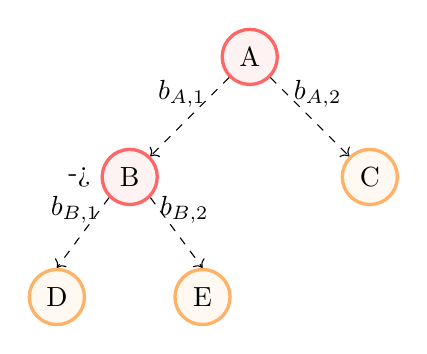
\begin{tikzpicture}
  \node[node, red] (node1) {A};
  \node[node, red, label=left:{->}] (node2) [below left=of node1] {B};
  \node[node, orange] (node3) [below right=of node1] {C};
  \node[node, orange] (node4) [below left=of node2, xshift=0.6cm] {D};
  \node[node, orange] (node5) [below right=of node2, xshift=-0.6cm] {E};

  \draw[dashed, ->] (node1.south west) -- (node2.north east) node[midway, above, xshift=-0.1cm] {$b_{A,1}$};
  \draw[dashed, ->] (node1.south east) -- (node3.north west) node[midway, above, xshift=0.1cm] {$b_{A,2}$};
  \draw[dashed, ->] (node2.south west) -- (node4.north) node[midway, above, xshift=-0.1cm] {$b_{B,1}$};
  \draw[dashed, ->] (node2.south east) -- (node5.north) node[midway, above, xshift=0.1cm] {$b_{B,2}$};

\end{tikzpicture}
\end{center}
\end{minipage}
\begin{minipage}{.5\textwidth}
\begin{center}

\vspace{0.3cm}
Promise Tree

\vspace{0.3cm}
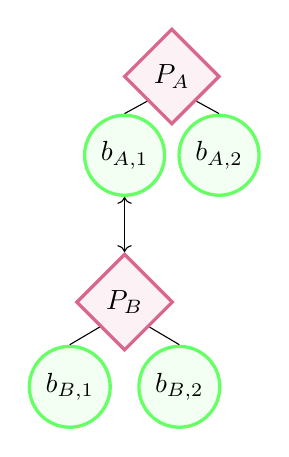
\begin{tikzpicture}
  \node[diamondnode, purple] (node1) {$P_A$};
  \node[node] (node2) [yshift=-1.0cm, xshift=-0.6cm] {$b_{A,1}$};
  \node[node] (node3) [yshift=-1.0cm, xshift=0.6cm] {$b_{A,2}$};
  \node[diamondnode, purple] (node4) [below=of node2, yshift=0.3cm] {$P_B$};
  \node[node] (node5) [below left=of node4, yshift=0.62cm, xshift=1.0cm] {$b_{B,1}$};
  \node[node] (node6) [below right=of node4, yshift=0.62cm, xshift=-1.0cm] {$b_{B,2}$};

  \draw (node1.south west) -- (node2.north);
  \draw (node1.south east) -- (node3.north);
  \draw[<->] (node2.south) -- (node4.north);
  \draw (node4.south west) -- (node5.north);
  \draw (node4.south east) -- (node6.north);
\end{tikzpicture}
\end{center}
\end{minipage}

Assume that D, E, C are the first Arg Nodes encountered by branches $b_{B,1}$, $b_{B,2}$, and $b_{A,2}$, respectively, and that they are traversed in such order.
Traversing D causes $b_{B,1}$ to forward chain the activation upwards. We colour Promise Tree objects teal when forward chaining has occurred through them.
Since $P_B$ is still not in Complete state after this step, we enqueue D and stall relevance propagation along its path.

\begin{minipage}{.5\textwidth}
\begin{center}

\vspace{0.3cm}
Computation Graph

\vspace{0.3cm}
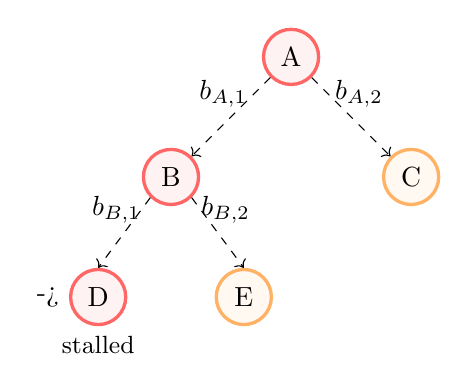
\begin{tikzpicture}
  \node[node, red] (node1) {A};
  \node[node, red] (node2) [below left=of node1] {B};
  \node[node, orange] (node3) [below right=of node1] {C};
  \node[node, red, label=below:{\small stalled}, label=left:{->}] (node4) [below left=of node2, xshift=0.6cm] {D};
  \node[node, orange] (node5) [below right=of node2, xshift=-0.6cm] {E};

  \draw[dashed, ->] (node1.south west) -- (node2.north east) node[midway, above, xshift=-0.1cm] {$b_{A,1}$};
  \draw[dashed, ->] (node1.south east) -- (node3.north west) node[midway, above, xshift=0.1cm] {$b_{A,2}$};
  \draw[dashed, ->] (node2.south west) -- (node4.north) node[midway, above, xshift=-0.1cm] {$b_{B,1}$};
  \draw[dashed, ->] (node2.south east) -- (node5.north) node[midway, above, xshift=0.1cm] {$b_{B,2}$};

\end{tikzpicture}
\end{center}
\end{minipage}
\begin{minipage}{.5\textwidth}
\begin{center}

\vspace{0.3cm}
Promise Tree

\vspace{0.3cm}
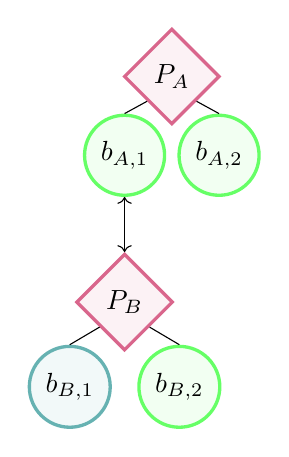
\begin{tikzpicture}
  \node[diamondnode, purple] (node1) {$P_A$};
  \node[node] (node2) [yshift=-1.0cm, xshift=-0.6cm] {$b_{A,1}$};
  \node[node] (node3) [yshift=-1.0cm, xshift=0.6cm] {$b_{A,2}$};
  \node[diamondnode, purple] (node4) [below=of node2, yshift=0.3cm] {$P_B$};
  \node[node, teal] (node5) [below left=of node4, yshift=0.62cm, xshift=1.0cm] {$b_{B,1}$};
  \node[node] (node6) [below right=of node4, yshift=0.62cm, xshift=-1.0cm] {$b_{B,2}$};

  \draw (node1.south west) -- (node2.north);
  \draw (node1.south east) -- (node3.north);
  \draw[<->] (node2.south) -- (node4.north);
  \draw (node4.south west) -- (node5.north);
  \draw (node4.south east) -- (node6.north);
\end{tikzpicture}
\end{center}
\end{minipage}

Likewise, once E is traversed, it will provide its forward output to $b_{B,2}$ to forward chain upwards. Since all branches of $P_B$ will have
forwarded their arguments, $P_B$ is now in Ready state.

\begin{minipage}{.5\textwidth}
\begin{center}

\vspace{0.3cm}
Computation Graph

\vspace{0.3cm}
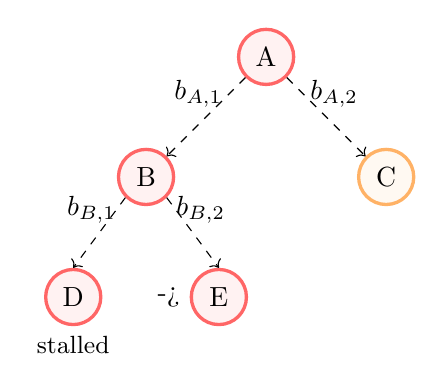
\begin{tikzpicture}
  \node[node, red] (node1) {A};
  \node[node, red] (node2) [below left=of node1] {B};
  \node[node, orange] (node3) [below right=of node1] {C};
  \node[node, red, label=below:{\small stalled}] (node4) [below left=of node2, xshift=0.6cm] {D};
  \node[node, red, label=left:{->}] (node5) [below right=of node2, xshift=-0.6cm] {E};

  \draw[dashed, ->] (node1.south west) -- (node2.north east) node[midway, above, xshift=-0.1cm] {$b_{A,1}$};
  \draw[dashed, ->] (node1.south east) -- (node3.north west) node[midway, above, xshift=0.1cm] {$b_{A,2}$};
  \draw[dashed, ->] (node2.south west) -- (node4.north) node[midway, above, xshift=-0.1cm] {$b_{B,1}$};
  \draw[dashed, ->] (node2.south east) -- (node5.north) node[midway, above, xshift=0.1cm] {$b_{B,2}$};

\end{tikzpicture}
\end{center}
\end{minipage}
\begin{minipage}{.5\textwidth}
\begin{center}

\vspace{0.3cm}
Promise Tree

\vspace{0.3cm}
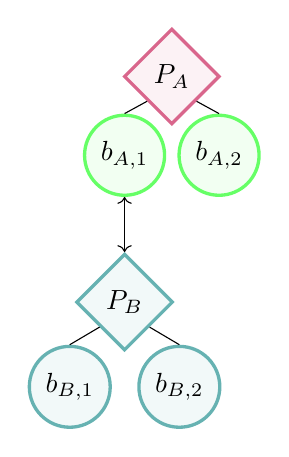
\begin{tikzpicture}
  \node[diamondnode, purple] (node1) {$P_A$};
  \node[node] (node2) [yshift=-1.0cm, xshift=-0.6cm] {$b_{A,1}$};
  \node[node] (node3) [yshift=-1.0cm, xshift=0.6cm] {$b_{A,2}$};
  \node[diamondnode, teal] (node4) [below=of node2, yshift=0.3cm] {$P_B$};
  \node[node, teal] (node5) [below left=of node4, yshift=0.62cm, xshift=1.0cm] {$b_{B,1}$};
  \node[node, teal] (node6) [below right=of node4, yshift=0.62cm, xshift=-1.0cm] {$b_{B,2}$};

  \draw (node1.south west) -- (node2.north);
  \draw (node1.south east) -- (node3.north);
  \draw[<->] (node2.south) -- (node4.north);
  \draw (node4.south west) -- (node5.north);
  \draw (node4.south east) -- (node6.north);
\end{tikzpicture}
\end{center}
\end{minipage}

When a Promise becomes Ready, this triggers the first half of the Promise Tree resolution at that Promise. It will apply its characteristic
operation using the results materialized by its branches' forward chains as inputs, and pass this output to its parents in the Promise Tree by
calling \texttt{parent.setarg(self.op\_result)}.

However, after this step, $P_B$ is still not in Complete state, so we must also enqueue E and stall relevance propagation along this path.

\begin{minipage}{.5\textwidth}
\begin{center}

\vspace{0.3cm}
Computation Graph

\vspace{0.3cm}
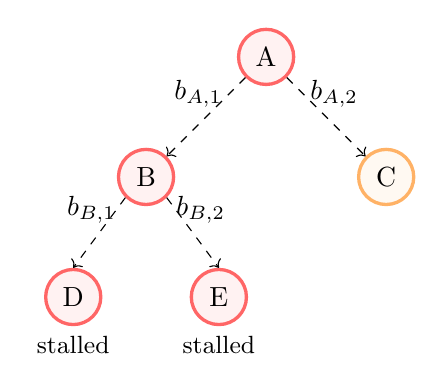
\begin{tikzpicture}
  \node[node, red] (node1) {A};
  \node[node, red] (node2) [below left=of node1] {B};
  \node[node, orange] (node3) [below right=of node1] {C};
  \node[node, red, label=below:{\small stalled}] (node4) [below left=of node2, xshift=0.6cm] {D};
  \node[node, red, label=below:{\small stalled}] (node5) [below right=of node2, xshift=-0.6cm] {E};

  \draw[dashed, ->] (node1.south west) -- (node2.north east) node[midway, above, xshift=-0.1cm] {$b_{A,1}$};
  \draw[dashed, ->] (node1.south east) -- (node3.north west) node[midway, above, xshift=0.1cm] {$b_{A,2}$};
  \draw[dashed, ->] (node2.south west) -- (node4.north) node[midway, above, xshift=-0.1cm] {$b_{B,1}$};
  \draw[dashed, ->] (node2.south east) -- (node5.north) node[midway, above, xshift=0.1cm] {$b_{B,2}$};

\end{tikzpicture}
\end{center}
\end{minipage}
\begin{minipage}{.5\textwidth}
\begin{center}

\vspace{0.3cm}
Promise Tree

\vspace{0.3cm}
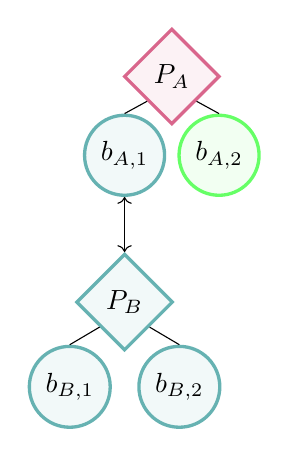
\begin{tikzpicture}
  \node[diamondnode, purple] (node1) {$P_A$};
  \node[node, teal] (node2) [yshift=-1.0cm, xshift=-0.6cm] {$b_{A,1}$};
  \node[node] (node3) [yshift=-1.0cm, xshift=0.6cm] {$b_{A,2}$};
  \node[diamondnode, teal] (node4) [below=of node2, yshift=0.3cm] {$P_B$};
  \node[node, teal] (node5) [below left=of node4, yshift=0.62cm, xshift=1.0cm] {$b_{B,1}$};
  \node[node, teal] (node6) [below right=of node4, yshift=0.62cm, xshift=-1.0cm] {$b_{B,2}$};

  \draw (node1.south west) -- (node2.north);
  \draw (node1.south east) -- (node3.north);
  \draw[<->] (node2.south) -- (node4.north);
  \draw (node4.south west) -- (node5.north);
  \draw (node4.south east) -- (node6.north);
\end{tikzpicture}
\end{center}
\end{minipage}

Now, when C is traversed, the pattern repeats. $b_{A,2}$ will forward-chain the activation from C, and it will cause $P_A$ to reach Ready state.

\begin{minipage}{.5\textwidth}
\begin{center}

\vspace{0.3cm}
Computation Graph

\vspace{0.3cm}
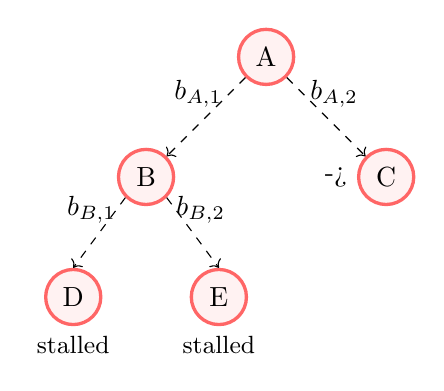
\begin{tikzpicture}
  \node[node, red] (node1) {A};
  \node[node, red] (node2) [below left=of node1] {B};
  \node[node, red, label=left:{->}] (node3) [below right=of node1] {C};
  \node[node, red, label=below:{\small stalled}] (node4) [below left=of node2, xshift=0.6cm] {D};
  \node[node, red, label=below:{\small stalled}] (node5) [below right=of node2, xshift=-0.6cm] {E};

  \draw[dashed, ->] (node1.south west) -- (node2.north east) node[midway, above, xshift=-0.1cm] {$b_{A,1}$};
  \draw[dashed, ->] (node1.south east) -- (node3.north west) node[midway, above, xshift=0.1cm] {$b_{A,2}$};
  \draw[dashed, ->] (node2.south west) -- (node4.north) node[midway, above, xshift=-0.1cm] {$b_{B,1}$};
  \draw[dashed, ->] (node2.south east) -- (node5.north) node[midway, above, xshift=0.1cm] {$b_{B,2}$};

\end{tikzpicture}
\end{center}
\end{minipage}
\begin{minipage}{.5\textwidth}
\begin{center}

\vspace{0.3cm}
Promise Tree

\vspace{0.3cm}
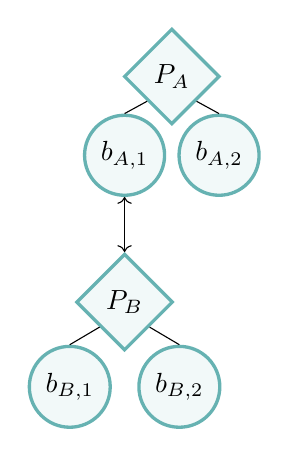
\begin{tikzpicture}
  \node[diamondnode, teal] (node1) {$P_A$};
  \node[node, teal] (node2) [yshift=-1.0cm, xshift=-0.6cm] {$b_{A,1}$};
  \node[node, teal] (node3) [yshift=-1.0cm, xshift=0.6cm] {$b_{A,2}$};
  \node[diamondnode, teal] (node4) [below=of node2, yshift=0.3cm] {$P_B$};
  \node[node, teal] (node5) [below left=of node4, yshift=0.62cm, xshift=1.0cm] {$b_{B,1}$};
  \node[node, teal] (node6) [below right=of node4, yshift=0.62cm, xshift=-1.0cm] {$b_{B,2}$};

  \draw (node1.south west) -- (node2.north);
  \draw (node1.south east) -- (node3.north);
  \draw[<->] (node2.south) -- (node4.north);
  \draw (node4.south west) -- (node5.north);
  \draw (node4.south east) -- (node6.north);
\end{tikzpicture}
\end{center}
\end{minipage}

And since $P_A$ has no parents in the Promise Tree, it will now begin the backpropagation of relevance, now that all arguments have been resolved.
It will do this for all of its own branches using the backward chains stored within them, and recursively do so for the children of those branches.

We also colour nodes in the Promise Tree as blue when relevance has been propagated through them.

Since this all occurs in one step, we label the order in which propagation occurs at each node in both the Computation Graph and Promise Tree.

\begin{minipage}{.5\textwidth}
\begin{center}

\vspace{0.3cm}
Computation Graph

\vspace{0.3cm}
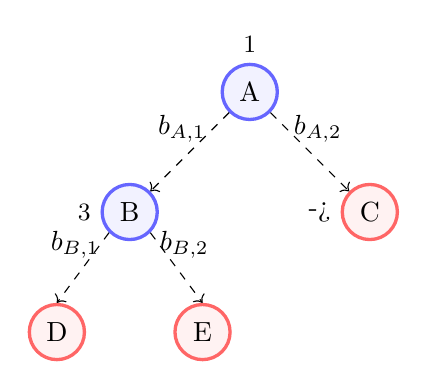
\begin{tikzpicture}
  \node[node, blue, label={\small 1}] (node1) {A};
  \node[node, blue, label=left:{\small 3}] (node2) [below left=of node1] {B};
  \node[node, red, label=left:{->}] (node3) [below right=of node1] {C};
  \node[node, red] (node4) [below left=of node2, xshift=0.6cm] {D};
  \node[node, red] (node5) [below right=of node2, xshift=-0.6cm] {E};

  \draw[dashed, ->] (node1.south west) -- (node2.north east) node[midway, above, xshift=-0.1cm] {$b_{A,1}$};
  \draw[dashed, ->] (node1.south east) -- (node3.north west) node[midway, above, xshift=0.1cm] {$b_{A,2}$};
  \draw[dashed, ->] (node2.south west) -- (node4.north) node[midway, above, xshift=-0.1cm] {$b_{B,1}$};
  \draw[dashed, ->] (node2.south east) -- (node5.north) node[midway, above, xshift=0.1cm] {$b_{B,2}$};

\end{tikzpicture}
\end{center}
\end{minipage}
\begin{minipage}{.5\textwidth}
\begin{center}

\vspace{0.3cm}
Promise Tree

\vspace{0.3cm}
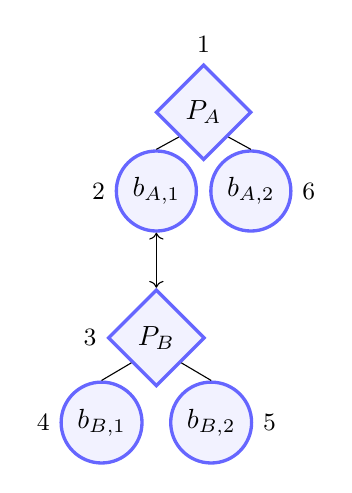
\begin{tikzpicture}
  \node[diamondnode, blue, label={\small 1}] (node1) {$P_A$};
  \node[node, blue, label=left:{\small 2}] (node2) [yshift=-1.0cm, xshift=-0.6cm] {$b_{A,1}$};
  \node[node, blue, label=right:{\small 6}] (node3) [yshift=-1.0cm, xshift=0.6cm] {$b_{A,2}$};
  \node[diamondnode, blue, label=left:{\small 3}] (node4) [below=of node2, yshift=0.3cm] {$P_B$};
  \node[node, blue, label=left:{\small 4}] (node5) [below left=of node4, yshift=0.62cm, xshift=1.0cm] {$b_{B,1}$};
  \node[node, blue, label=right:{\small 5}] (node6) [below right=of node4, yshift=0.62cm, xshift=-1.0cm] {$b_{B,2}$};

  \draw (node1.south west) -- (node2.north);
  \draw (node1.south east) -- (node3.north);
  \draw[<->] (node2.south) -- (node4.north);
  \draw (node4.south west) -- (node5.north);
  \draw (node4.south east) -- (node6.north);
\end{tikzpicture}
\end{center}
\end{minipage}

Note that although the relevance has propagated through the Promise Branches $b_{A,2}$, $b_{B,1}$, and $b_{B,2}$, the propagation functions
of the nodes at the end of their chains, D, E, C, respectively, have not been called at this moment, thus we do not say that relevance
has been propagated through them yet. Their propagation will resume in further iterations using the relevances passed to them through
those branches.

And see that the traversal pointer has remained at C, so we simply continue propagating along its path.
Also, since $P_B$ is Complete, D and E will also be dequeued in coming iterations to continue propagation.

\begin{minipage}{.5\textwidth}
\begin{center}

\vspace{0.3cm}
Computation Graph

\vspace{0.3cm}
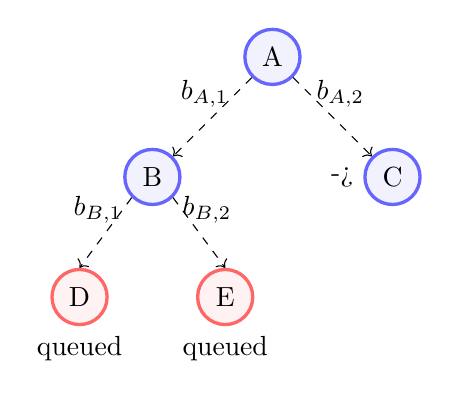
\begin{tikzpicture}
  \node[node, blue] (node1) {A};
  \node[node, blue] (node2) [below left=of node1] {B};
  \node[node, blue, label=left:{->}] (node3) [below right=of node1] {C};
  \node[node, red, label=below:{queued}] (node4) [below left=of node2, xshift=0.6cm] {D};
  \node[node, red, label=below:{queued}] (node5) [below right=of node2, xshift=-0.6cm] {E};

  \draw[dashed, ->] (node1.south west) -- (node2.north east) node[midway, above, xshift=-0.1cm] {$b_{A,1}$};
  \draw[dashed, ->] (node1.south east) -- (node3.north west) node[midway, above, xshift=0.1cm] {$b_{A,2}$};
  \draw[dashed, ->] (node2.south west) -- (node4.north) node[midway, above, xshift=-0.1cm] {$b_{B,1}$};
  \draw[dashed, ->] (node2.south east) -- (node5.north) node[midway, above, xshift=0.1cm] {$b_{B,2}$};

\end{tikzpicture}
\end{center}
\end{minipage}
\begin{minipage}{.5\textwidth}
\begin{center}

\vspace{0.3cm}
Promise Tree

\vspace{0.3cm}
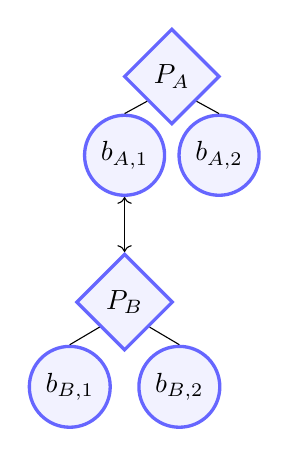
\begin{tikzpicture}
  \node[diamondnode, blue] (node1) {$P_A$};
  \node[node, blue] (node2) [yshift=-1.0cm, xshift=-0.6cm] {$b_{A,1}$};
  \node[node, blue] (node3) [yshift=-1.0cm, xshift=0.6cm] {$b_{A,2}$};
  \node[diamondnode, blue] (node4) [below=of node2, yshift=0.3cm] {$P_B$};
  \node[node, blue] (node5) [below left=of node4, yshift=0.62cm, xshift=1.0cm] {$b_{B,1}$};
  \node[node, blue] (node6) [below right=of node4, yshift=0.62cm, xshift=-1.0cm] {$b_{B,2}$};

  \draw (node1.south west) -- (node2.north);
  \draw (node1.south east) -- (node3.north);
  \draw[<->] (node2.south) -- (node4.north);
  \draw (node4.south west) -- (node5.north);
  \draw (node4.south east) -- (node6.north);
\end{tikzpicture}
\end{center}
\end{minipage}

\begin{minipage}{.5\textwidth}
\begin{center}

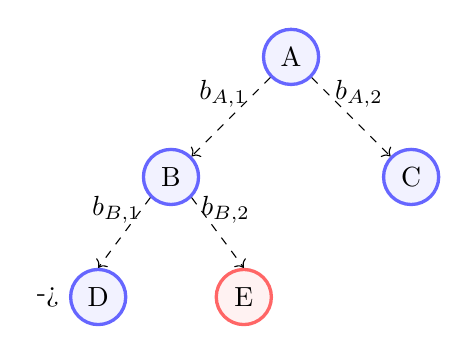
\begin{tikzpicture}
  \node[node, blue] (node1) {A};
  \node[node, blue] (node2) [below left=of node1] {B};
  \node[node, blue] (node3) [below right=of node1] {C};
  \node[node, blue, label=left:{->}] (node4) [below left=of node2, xshift=0.6cm] {D};
  \node[node, red] (node5) [below right=of node2, xshift=-0.6cm] {E};

  \draw[dashed, ->] (node1.south west) -- (node2.north east) node[midway, above, xshift=-0.1cm] {$b_{A,1}$};
  \draw[dashed, ->] (node1.south east) -- (node3.north west) node[midway, above, xshift=0.1cm] {$b_{A,2}$};
  \draw[dashed, ->] (node2.south west) -- (node4.north) node[midway, above, xshift=-0.1cm] {$b_{B,1}$};
  \draw[dashed, ->] (node2.south east) -- (node5.north) node[midway, above, xshift=0.1cm] {$b_{B,2}$};

\end{tikzpicture}
\end{center}
\end{minipage}
\begin{minipage}{.5\textwidth}
\begin{center}

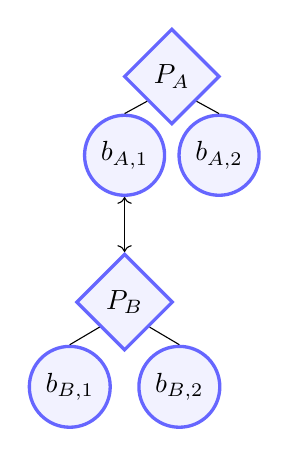
\begin{tikzpicture}
  \node[diamondnode, blue] (node1) {$P_A$};
  \node[node, blue] (node2) [yshift=-1.0cm, xshift=-0.6cm] {$b_{A,1}$};
  \node[node, blue] (node3) [yshift=-1.0cm, xshift=0.6cm] {$b_{A,2}$};
  \node[diamondnode, blue] (node4) [below=of node2, yshift=0.3cm] {$P_B$};
  \node[node, blue] (node5) [below left=of node4, yshift=0.62cm, xshift=1.0cm] {$b_{B,1}$};
  \node[node, blue] (node6) [below right=of node4, yshift=0.62cm, xshift=-1.0cm] {$b_{B,2}$};

  \draw (node1.south west) -- (node2.north);
  \draw (node1.south east) -- (node3.north);
  \draw[<->] (node2.south) -- (node4.north);
  \draw (node4.south west) -- (node5.north);
  \draw (node4.south east) -- (node6.north);
\end{tikzpicture}
\end{center}
\end{minipage}

\begin{minipage}{.5\textwidth}
\begin{center}

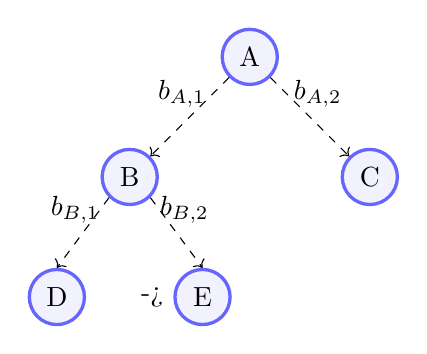
\begin{tikzpicture}
  \node[node, blue] (node1) {A};
  \node[node, blue] (node2) [below left=of node1] {B};
  \node[node, blue] (node3) [below right=of node1] {C};
  \node[node, blue] (node4) [below left=of node2, xshift=0.6cm] {D};
  \node[node, blue, label=left:{->}] (node5) [below right=of node2, xshift=-0.6cm] {E};

  \draw[dashed, ->] (node1.south west) -- (node2.north east) node[midway, above, xshift=-0.1cm] {$b_{A,1}$};
  \draw[dashed, ->] (node1.south east) -- (node3.north west) node[midway, above, xshift=0.1cm] {$b_{A,2}$};
  \draw[dashed, ->] (node2.south west) -- (node4.north) node[midway, above, xshift=-0.1cm] {$b_{B,1}$};
  \draw[dashed, ->] (node2.south east) -- (node5.north) node[midway, above, xshift=0.1cm] {$b_{B,2}$};

\end{tikzpicture}
\end{center}
\end{minipage}
\begin{minipage}{.5\textwidth}
\begin{center}

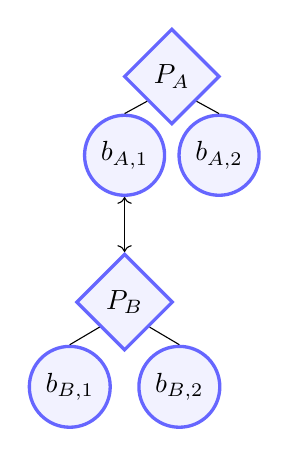
\begin{tikzpicture}
  \node[diamondnode, blue] (node1) {$P_A$};
  \node[node, blue] (node2) [yshift=-1.0cm, xshift=-0.6cm] {$b_{A,1}$};
  \node[node, blue] (node3) [yshift=-1.0cm, xshift=0.6cm] {$b_{A,2}$};
  \node[diamondnode, blue] (node4) [below=of node2, yshift=0.3cm] {$P_B$};
  \node[node, blue] (node5) [below left=of node4, yshift=0.62cm, xshift=1.0cm] {$b_{B,1}$};
  \node[node, blue] (node6) [below right=of node4, yshift=0.62cm, xshift=-1.0cm] {$b_{B,2}$};

  \draw (node1.south west) -- (node2.north);
  \draw (node1.south east) -- (node3.north);
  \draw[<->] (node2.south) -- (node4.north);
  \draw (node4.south west) -- (node5.north);
  \draw (node4.south east) -- (node6.north);
\end{tikzpicture}
\end{center}
\end{minipage}

\subsection{Solution to Promise Deadlock: Pre-Promises}
\label{appendix:pre-promises}

The solution to Promise Deadlock is to allow Promise Branches to "reach ahead" past the traversal frontier to locate their Arg Nodes, without triggering full relevance backpropagation.

When a node $v$ receives a Promise Branch input $p_1$ but is still waiting for other inputs (i.e., landed inputs < in-degree), we instantiate a \textbf{Pre-Promise}, which only has one branch $p_2$, at $v$
(since it only has one branch, we simply refer to the Pre-Promise as its branch $p_2$). This Pre-Promise:

\begin{enumerate}
    \item Has a parent connection to $p_1$ (enabling forward-chaining of activations)
    \item Does NOT register as a child of $p_1$ (preventing backward-chaining of relevance)
    \item Continues traversal to find its Arg Node
\end{enumerate}

The parent-child asymmetry creates the desired behavior: $p_2$ can reach its Arg Node, forward-chain the activation back through its parent connection to satisfy $p_1$'s requirements, but relevance propagation is blocked at $v$ until the traversal heuristic naturally revisits it (when all inputs have landed).

Once $v$'s in-degree is satisfied later in the traversal:
\begin{itemize}
    \item The Pre-Promise $p_2$ is "promoted" by establishing its child connection to $p_1$
    \item If $p_1$'s Promise is now complete (all args resolved), backward-chaining proceeds
    \item The traversal continues normally from $p_2$'s Arg Node after backward-chaining.
\end{itemize}

To illustrate the function of Pre-Promises, we will pick up where the example in Section 4.3.3 left off. We have that D is trying to propagate a Promise Branch to E, but E does not
have all its inputs yet. Therefore, we create a Pre-Promise $p_3$, and allow traversal to continue at E, now giving $p_3$ as E's input from D.

\begin{center}
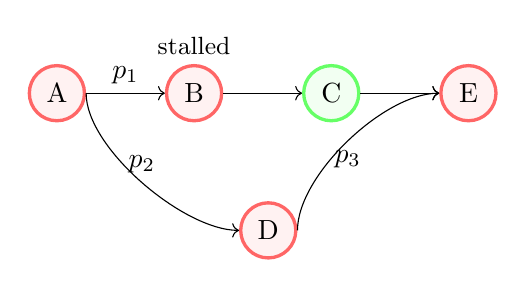
\begin{tikzpicture}
%Nodes
\node[node, red] (node1) {A};
\node[node, red, label={\small stalled}] (node2) [right=of node1] {B};
\node[node] (node3) [right=of node2] {C};
\node[node, red] (node4) [below=of node3, xshift=-8mm] {D};
\node[node, red] (node5) [right=of node3] {E};

%Lines
\draw[->] (node1.east) -- (node2.west) node[midway, above] {$p_1$};
\draw[->] (node2.east) -- (node3.west);
\draw[->] (node3.east) -- (node5.west);
\draw[->] (node1.east) .. controls +(down:7mm) and +(left:7mm) .. (node4.west) node[midway, above] {$p_2$};
\draw[->] (node4.east) .. controls +(up:7mm) and +(left:7mm) .. (node5.west) node[midway, below] {$p_3$};
\end{tikzpicture}
\end{center}

$p_3$ retrieves and forward-chains the activation at E to $p_2$, which then forward-chains it to obtain A's missing activation. We now have that A, B, D, E have gone through
forward-chaining. We colour them as teal to signify this.

\begin{center}
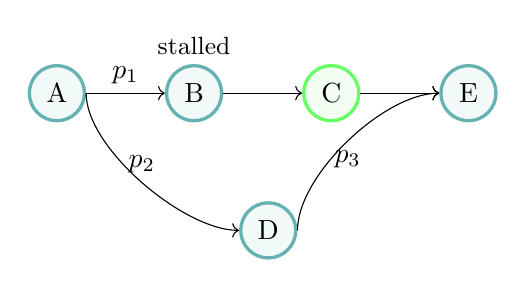
\begin{tikzpicture}
%Nodes
\node[node, teal] (node1) {A};
\node[node, teal, label={\small stalled}] (node2) [right=of node1] {B};
\node[node] (node3) [right=of node2] {C};
\node[node, teal] (node4) [below=of node3, xshift=-8mm] {D};
\node[node, teal] (node5) [right=of node3] {E};

%Lines
\draw[->] (node1.east) -- (node2.west) node[midway, above] {$p_1$};
\draw[->] (node2.east) -- (node3.west);
\draw[->] (node3.east) -- (node5.west);
\draw[->] (node1.east) .. controls +(down:7mm) and +(left:7mm) .. (node4.west) node[midway, above] {$p_2$};
\draw[->] (node4.east) .. controls +(up:7mm) and +(left:7mm) .. (node5.west) node[midway, below] {$p_3$};
\end{tikzpicture}
\end{center}

This is followed by $P$ triggering relevance backpropagation through all of its branches. Blue nodes signify that true relevance values have been propagated through them.
Crucially, E does not continue this propagation due to the lack of a child connection from $p_2$ to $p_3$.

\begin{center}
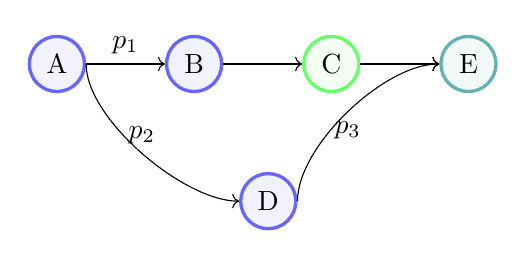
\begin{tikzpicture}
%Nodes
\node[node, blue] (node1) {A};
\node[node, blue] (node2) [right=of node1] {B};
\node[node] (node3) [right=of node2] {C};
\node[node, blue] (node4) [below=of node3, xshift=-8mm] {D};
\node[node, teal] (node5) [right=of node3] {E};

%Lines
\draw[->] (node1.east) -- (node2.west) node[midway, above] {$p_1$};
\draw[->] (node2.east) -- (node3.west);
\draw[->] (node3.east) -- (node5.west);
\draw[->] (node1.east) .. controls +(down:7mm) and +(left:7mm) .. (node4.west) node[midway, above] {$p_2$};
\draw[->] (node4.east) .. controls +(up:7mm) and +(left:7mm) .. (node5.west) node[midway, below] {$p_3$};
\end{tikzpicture}
\end{center}

Now, C is able to be traversed.

\begin{center}
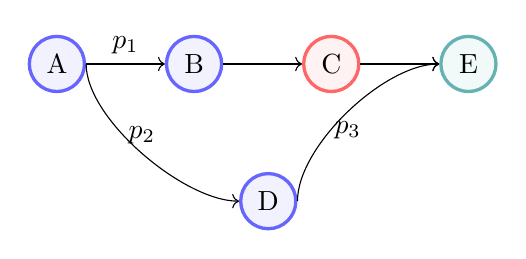
\begin{tikzpicture}
%Nodes
\node[node, blue] (node1) {A};
\node[node, blue] (node2) [right=of node1] {B};
\node[node, red] (node3) [right=of node2] {C};
\node[node, blue] (node4) [below=of node3, xshift=-8mm] {D};
\node[node, teal] (node5) [right=of node3] {E};

%Lines
\draw[->] (node1.east) -- (node2.west) node[midway, above] {$p_1$};
\draw[->] (node2.east) -- (node3.west);
\draw[->] (node3.east) -- (node5.west);
\draw[->] (node1.east) .. controls +(down:7mm) and +(left:7mm) .. (node4.west) node[midway, above] {$p_2$};
\draw[->] (node4.east) .. controls +(up:7mm) and +(left:7mm) .. (node5.west) node[midway, below] {$p_3$};
\end{tikzpicture}
\end{center}

And we propagate through it to E, finally.

\begin{center}
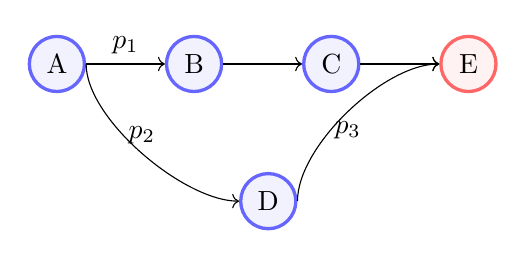
\begin{tikzpicture}
%Nodes
\node[node, blue] (node1) {A};
\node[node, blue] (node2) [right=of node1] {B};
\node[node, blue] (node3) [right=of node2] {C};
\node[node, blue] (node4) [below=of node3, xshift=-8mm] {D};
\node[node, red] (node5) [right=of node3] {E};

%Lines
\draw[->] (node1.east) -- (node2.west) node[midway, above] {$p_1$};
\draw[->] (node2.east) -- (node3.west);
\draw[->] (node3.east) -- (node5.west);
\draw[->] (node1.east) .. controls +(down:7mm) and +(left:7mm) .. (node4.west) node[midway, above] {$p_2$};
\draw[->] (node4.east) .. controls +(up:7mm) and +(left:7mm) .. (node5.west) node[midway, below] {$p_3$};
\end{tikzpicture}
\end{center}

\section{Input Aggregation}
When node $v$ receives multiple relevance inputs from in-neighbors, we aggregate before propagation:

\textbf{Tensor inputs} are typically summed element-wise: $R_v = \sum_{i=1}^k R_i$, but there are rare edge cases like when
propagating through a Split operation, where $R_v = concat(R_1 \ldots R_k)$, for example.

\textbf{Promise Branch inputs} $p_1, \ldots, p_k$ are merged into a single aggregation branch $p_{\text{agg}}$ with parent
connections to all $p_i$ but no child connections back. During forward-chaining, $p_{\text{agg}}$ distributes retrieved
activations to all parents. During backward-chaining, $p_{\text{agg}}$ sums relevances from all parents before continuing
propagation.

Notably, this kind of aggregation occurs naturally through the Pre-Promise mechanism. Consider that any such $v$ that
eventually receives more than one Promise Branch input, will at some point be in the exact state for requiring a
Pre-Promise ($|I| < \text{indegree}(v)$). This occurs right after $v$ receives its first Promise Branch input $p_1$.
As additional Promise Branches $p_2, \ldots, p_k$ arrive at $v$, they connect as parents to the Pre-Promise, and the
child connections are made when the Pre-Promise is promoted, completing the aggregation structure.

\textbf{Mixed Promise and Tensor inputs:} When $v$ receives both tensor relevances and Promise Branches, we handle Promise
aggregation as above. If only one Promise Branch is present, we still create a new aggregation branch $p_{\text{agg}}$ as
a child of the incoming branch. While this adds memory overhead, it maintains the Promise path abstraction required for
caching (\ref{sec:promise-caching}). If tensor relevances were allowed to merge directly into a Promise Branch's
internal nodes, cached Promise paths would behave incorrectly; relevance would be injected mid-chain rather than at the
Promise's Origin Node.

This process helps ensure that relevance is propagated only once through each node to prevent exponential blowup in graph
traversal and incorrect accumulation of relevance from multiple Promise Branches. This will help us prove Proposition 2:

\textbf{Proposition 2:} Each node in the computation graph has relevance propagated through it exactly once during LRP traversal.
\begin{proof}
  We prove this in two cases: standard propagation and Promise propagation.

  \textbf{Case 1: Standard Propagation.}
  By our traversal heuristic, and facilitated by the Input Aggregation process, we have that this statement will hold true in any case that
  follows the heuristic.

  By traversal heuristic, we process node $v$ only when all in-neighbors have propagated relevance to it. Since the
  computation graph is a DAG (no operation can depend on its own output), no traversal path starting from $v$ can return
  to $v$. 
  Input aggregation ensures that multiple incoming relevances are combined before processing, so $v$ is processed exactly
  once when all inputs arrive.

  \textbf{Case 2: Promise Propagation.}
  The two distinct phases of a Promise Branch are the forward chaining of activations when it reaches an Arg Node and the
  backward chaining of relevance, deferred until all parents in the Promise Tree are in Complete state.
  Therefore, even though the nodes within a Promise Branch path are traversed in the first phase, they do not have
  relevance propagated through them until the backward chain is executed, propagating all the way through to the Arg Node
  and skipping all internal nodes. Since the Arg Node is a descendent of $v$ and all internal nodes in the chain, by the
  DAG argument, none of those nodes can be revisited.

\end{proof}

\textbf{Claim:} The internal nodes of any two distinct Promise branches are disjoint.
\label{appendix:unique-chains}
\begin{proof}
  By Proposition 2 we have that no node has relevance propagated through it more than once in graph traversal.

  Suppose for contradiction that two distinct Promise branches $p_1$ and $p_2$ share an internal node $v$.
  However, this means that during traversal, both $p_1$ and $p_2$ had to traverse $v$, or else it would not be recorded in
  their chains. In that case, we would have applied Case 2 of Input Aggregation via the Pre-Promise mechanism, and both
  chains would then terminate at the creation of the Pre-Promise. But, this contradicts our premise that $v$ was an internal
  node for both branches, therefore it must be that no two distinct Promise branches share any internal nodes.
\end{proof}

\textbf{Remark.} This property ensures that the total number of nodes traversed by 
all Promises is bounded by $\delta = \sum_{v_p \in V_P} d(v_p) \leq |V|$, as stated 
in Theorem 1 (\ref{sec:lrp-complexity}). Each node contributes to at most one Promise's internal chain, preventing 
double-counting in complexity analysis.

\section{Attribution Faithfulness Evaluation Figures}

\begin{figure}[h]
  \centering
  \includegraphics[width=1.0\textwidth]{figures/VGG_attributions.png}
  \caption{Comparing methods for VGG attributions.}
\end{figure}


\begin{figure}[h]
  \centering
  \includegraphics[width=1.0\textwidth]{figures/vit_abpc_comparisons.png}
  \caption{Comparing faithfulness of methods using ABPC from pretrained ViT-b-16 performance on 1000 examples from the ImageNet CIFAR-10 test set. Occlusion is applied by replacing 16x16 patches with the corresponding regions from a Gaussian-blurred version of the image (kernel size = 51, $\sigma$ = 20). Red = MoRF curve, Blue = LeRF curve.}
\end{figure}

\end{document}
